\newpage

\subsection{Member Workflow Overview}
The system provides a comprehensive workflow for library members, enabling them to perform all essential library operations through an intuitive interface. Members can register for new accounts, search the library catalog, borrow and return books, and view their current loans and borrowing history. Figure \ref{fig:member_workflow} illustrates the complete member workflow, showing the various paths and operations available to registered users.

\begin{figure}[H]
	\centering
	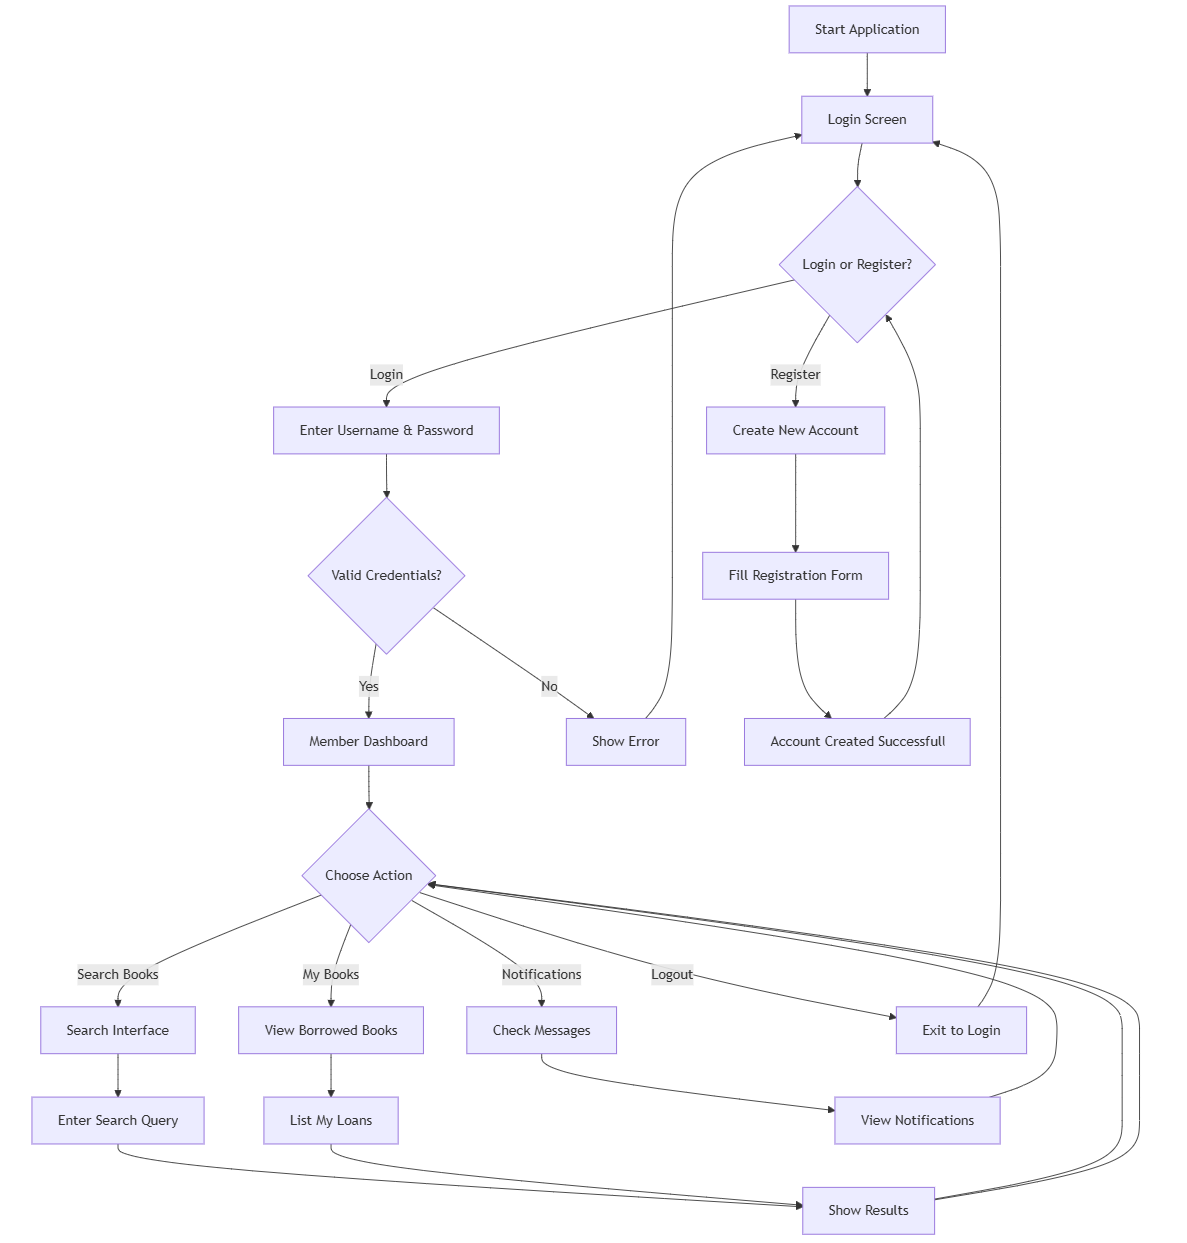
\includegraphics[width=\textwidth]{figures/member_workflow.png}
	\caption{Complete workflow diagram for library members.}
	\label{fig:member_workflow}
\end{figure}

\newpage

\subsection{Librarian Workflow Overview}
Librarians have access to administrative functions that enable them to manage the library's collection and oversee member activities. The librarian workflow includes adding new books to the catalog, updating book information, monitoring loan records, and managing member accounts. This administrative interface provides the tools necessary for effective library management. Figure \ref{fig:librarian_workflow} demonstrates the various administrative operations and decision points available to librarians.

\begin{figure}[H]
	\centering
	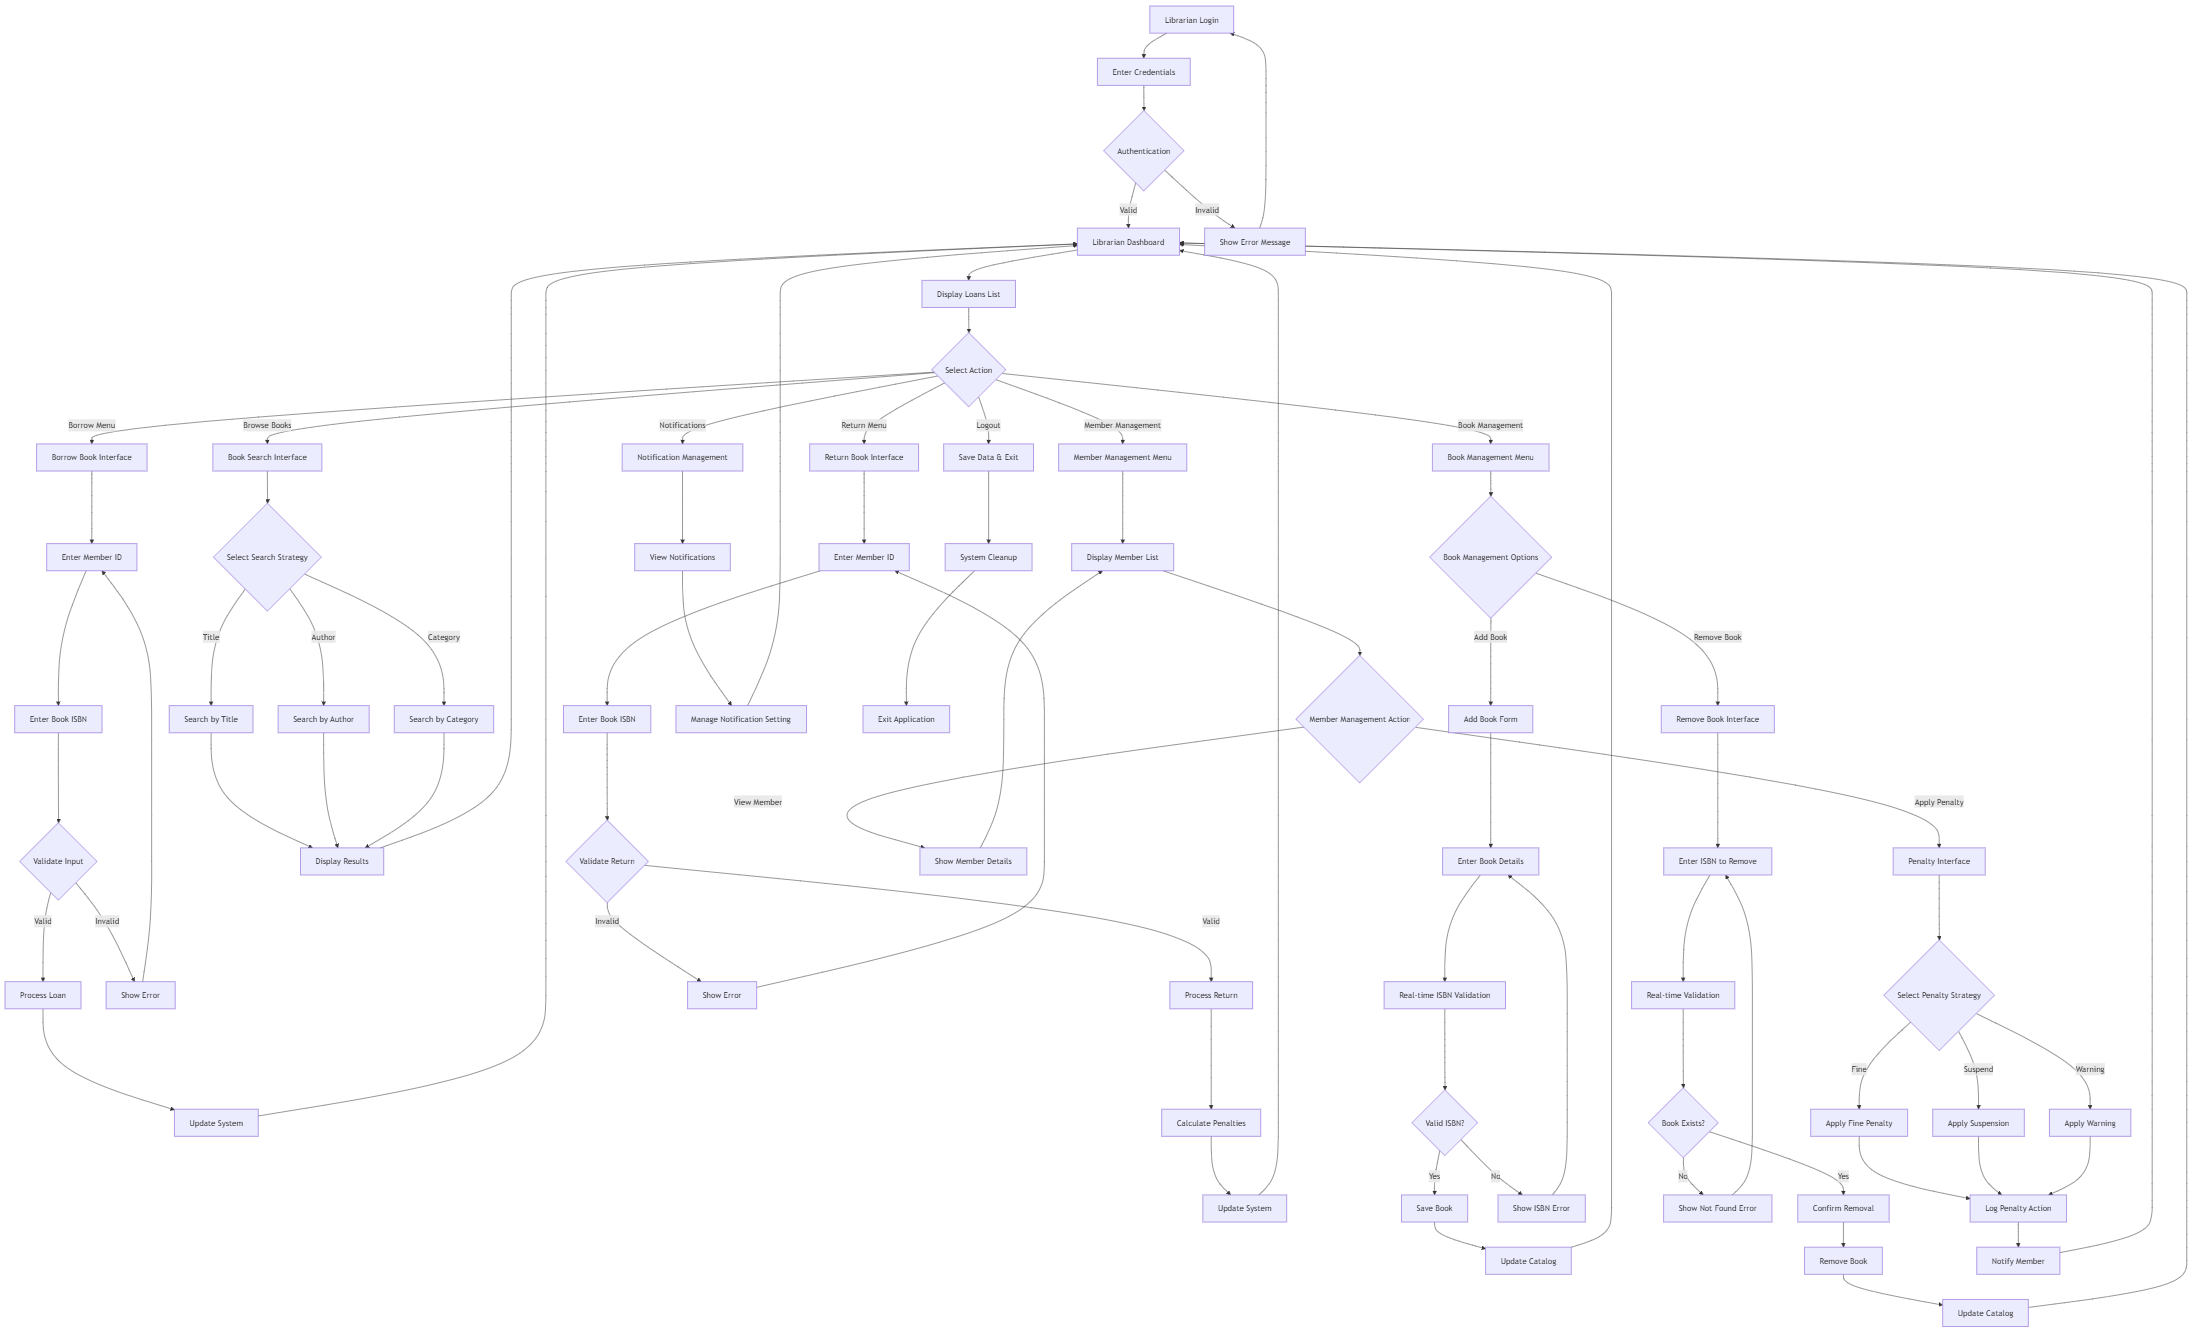
\includegraphics[width=\textwidth]{figures/librarian_workflow.png}
	\caption{Complete workflow diagram for library administrators.}
	\label{fig:librarian_workflow}
\end{figure}

\newpage

\subsection{Registering a New Member}
A new user interacts with the system to create a member account. The user selects the registration option from the main menu and provides the required credentials (username and password). The system then validates the input and creates a new member record, assigning a unique Member ID. The sequence of object interactions for this process is detailed in Figure \ref{fig:seq_register}.

\begin{figure}[H]
	\centering
	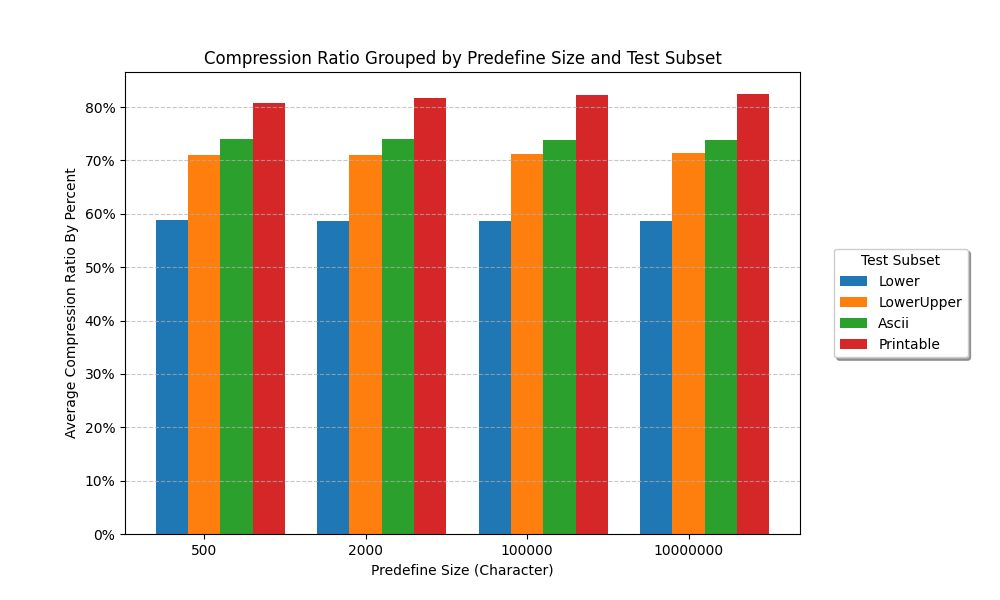
\includegraphics[width=\textwidth]{figures/sequence_register.png}
	\caption{Sequence Diagram for New Member Registration.}
	\label{fig:seq_register}
\end{figure}

\newpage

\subsection{Borrowing a Book}
A logged-in member can borrow a book from the library. The typical flow involves the member searching for a book and then selecting the "borrow" option, providing the book's ISBN. The system validates that the book is available, checks the member's borrowing eligibility, creates a new loan record, and finally updates the book's status. This workflow is visualized in Figure \ref{fig:seq_borrow}.

\begin{figure}[H]
	\centering
	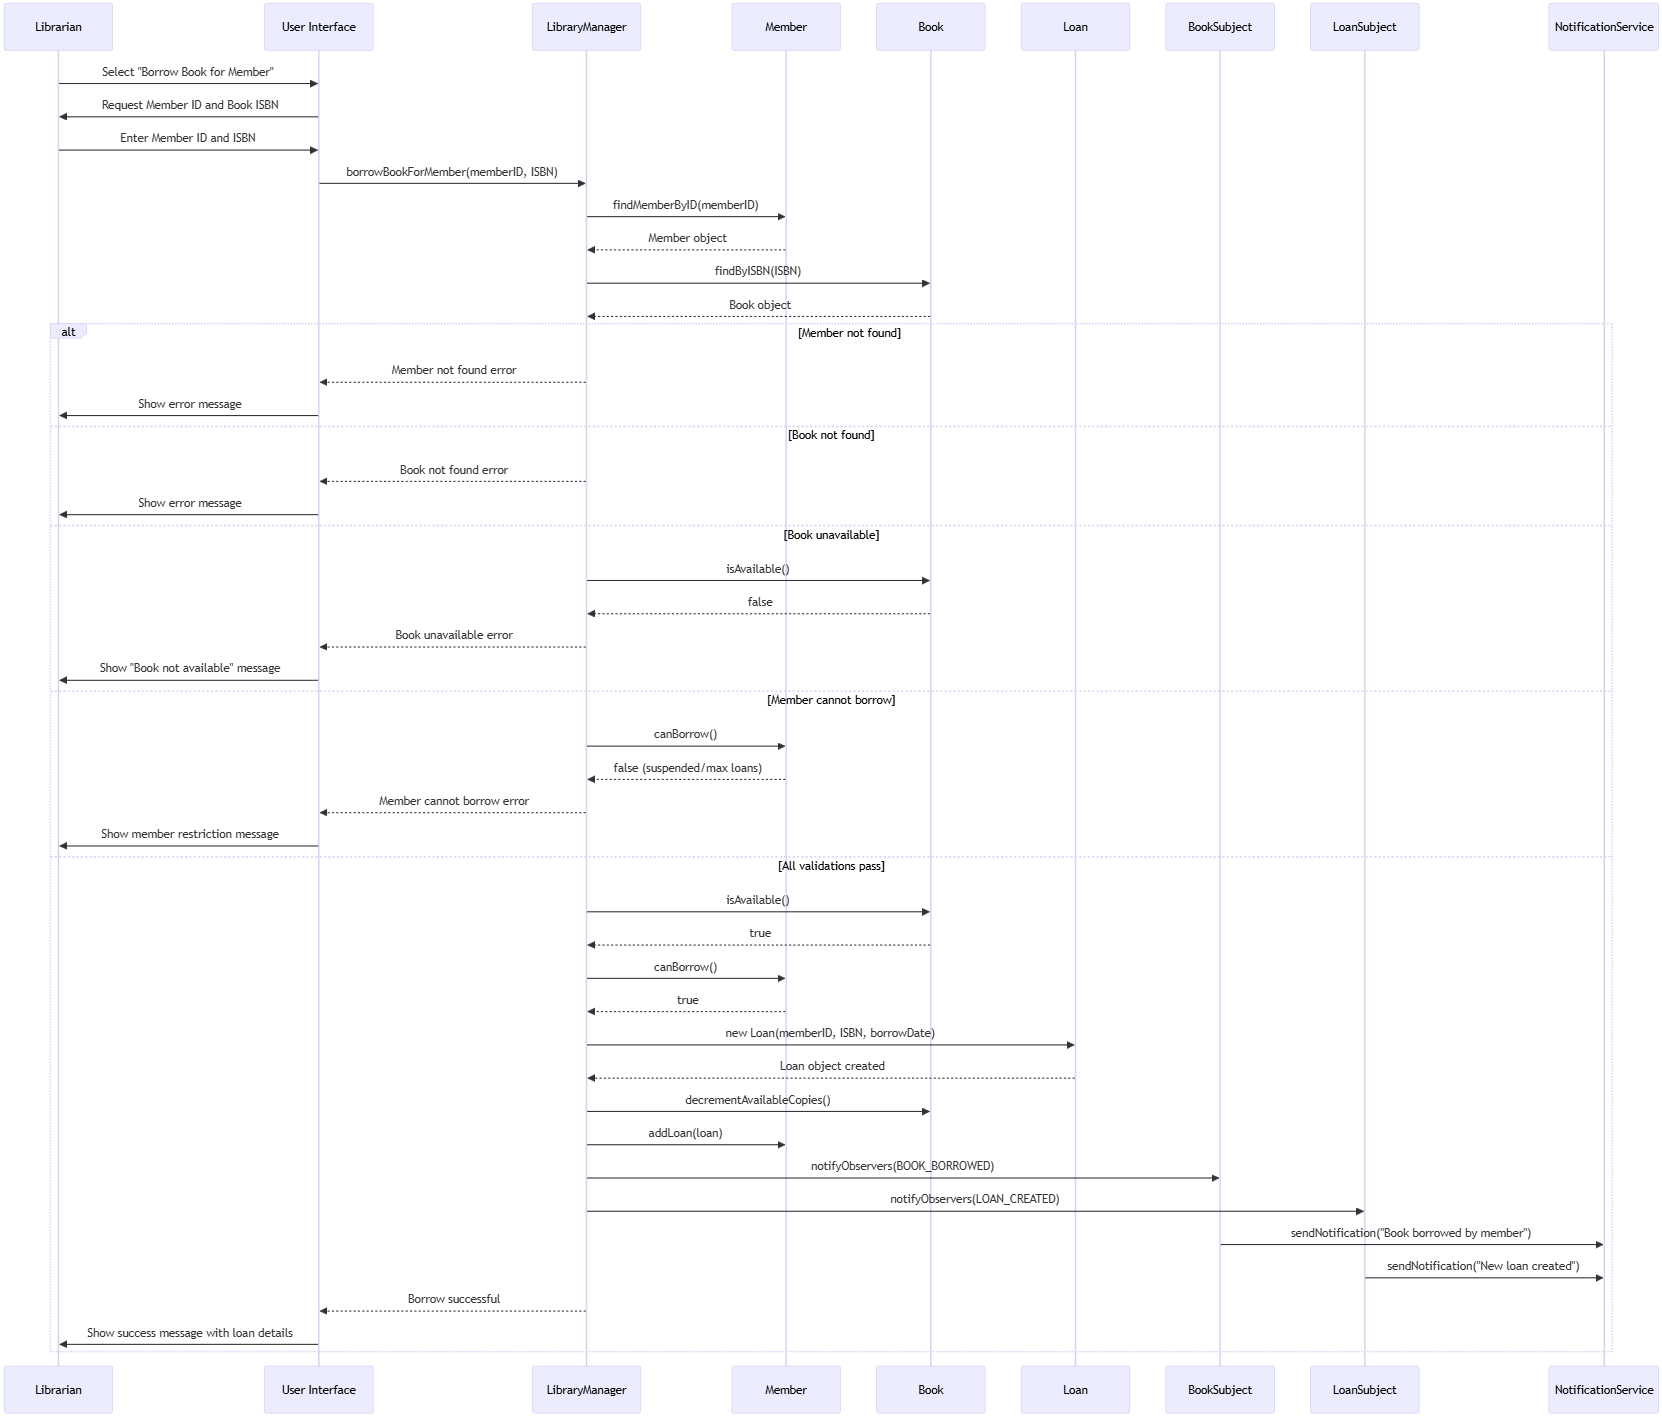
\includegraphics[width=\textwidth]{figures/sequence_borrow.png}
	\caption{Sequence Diagram for Borrowing a Book.}
	\label{fig:seq_borrow}
\end{figure}

\newpage

\subsection{Returning a Book}
When a member returns a book, they select the return option and provide the book's ISBN. The system finds the corresponding active loan record, updates its status to "returned," records the return date, and increments the number of available copies for that book. Figure \ref{fig:seq_return} illustrates the object interactions for this process.

\begin{figure}[H]
	\centering
	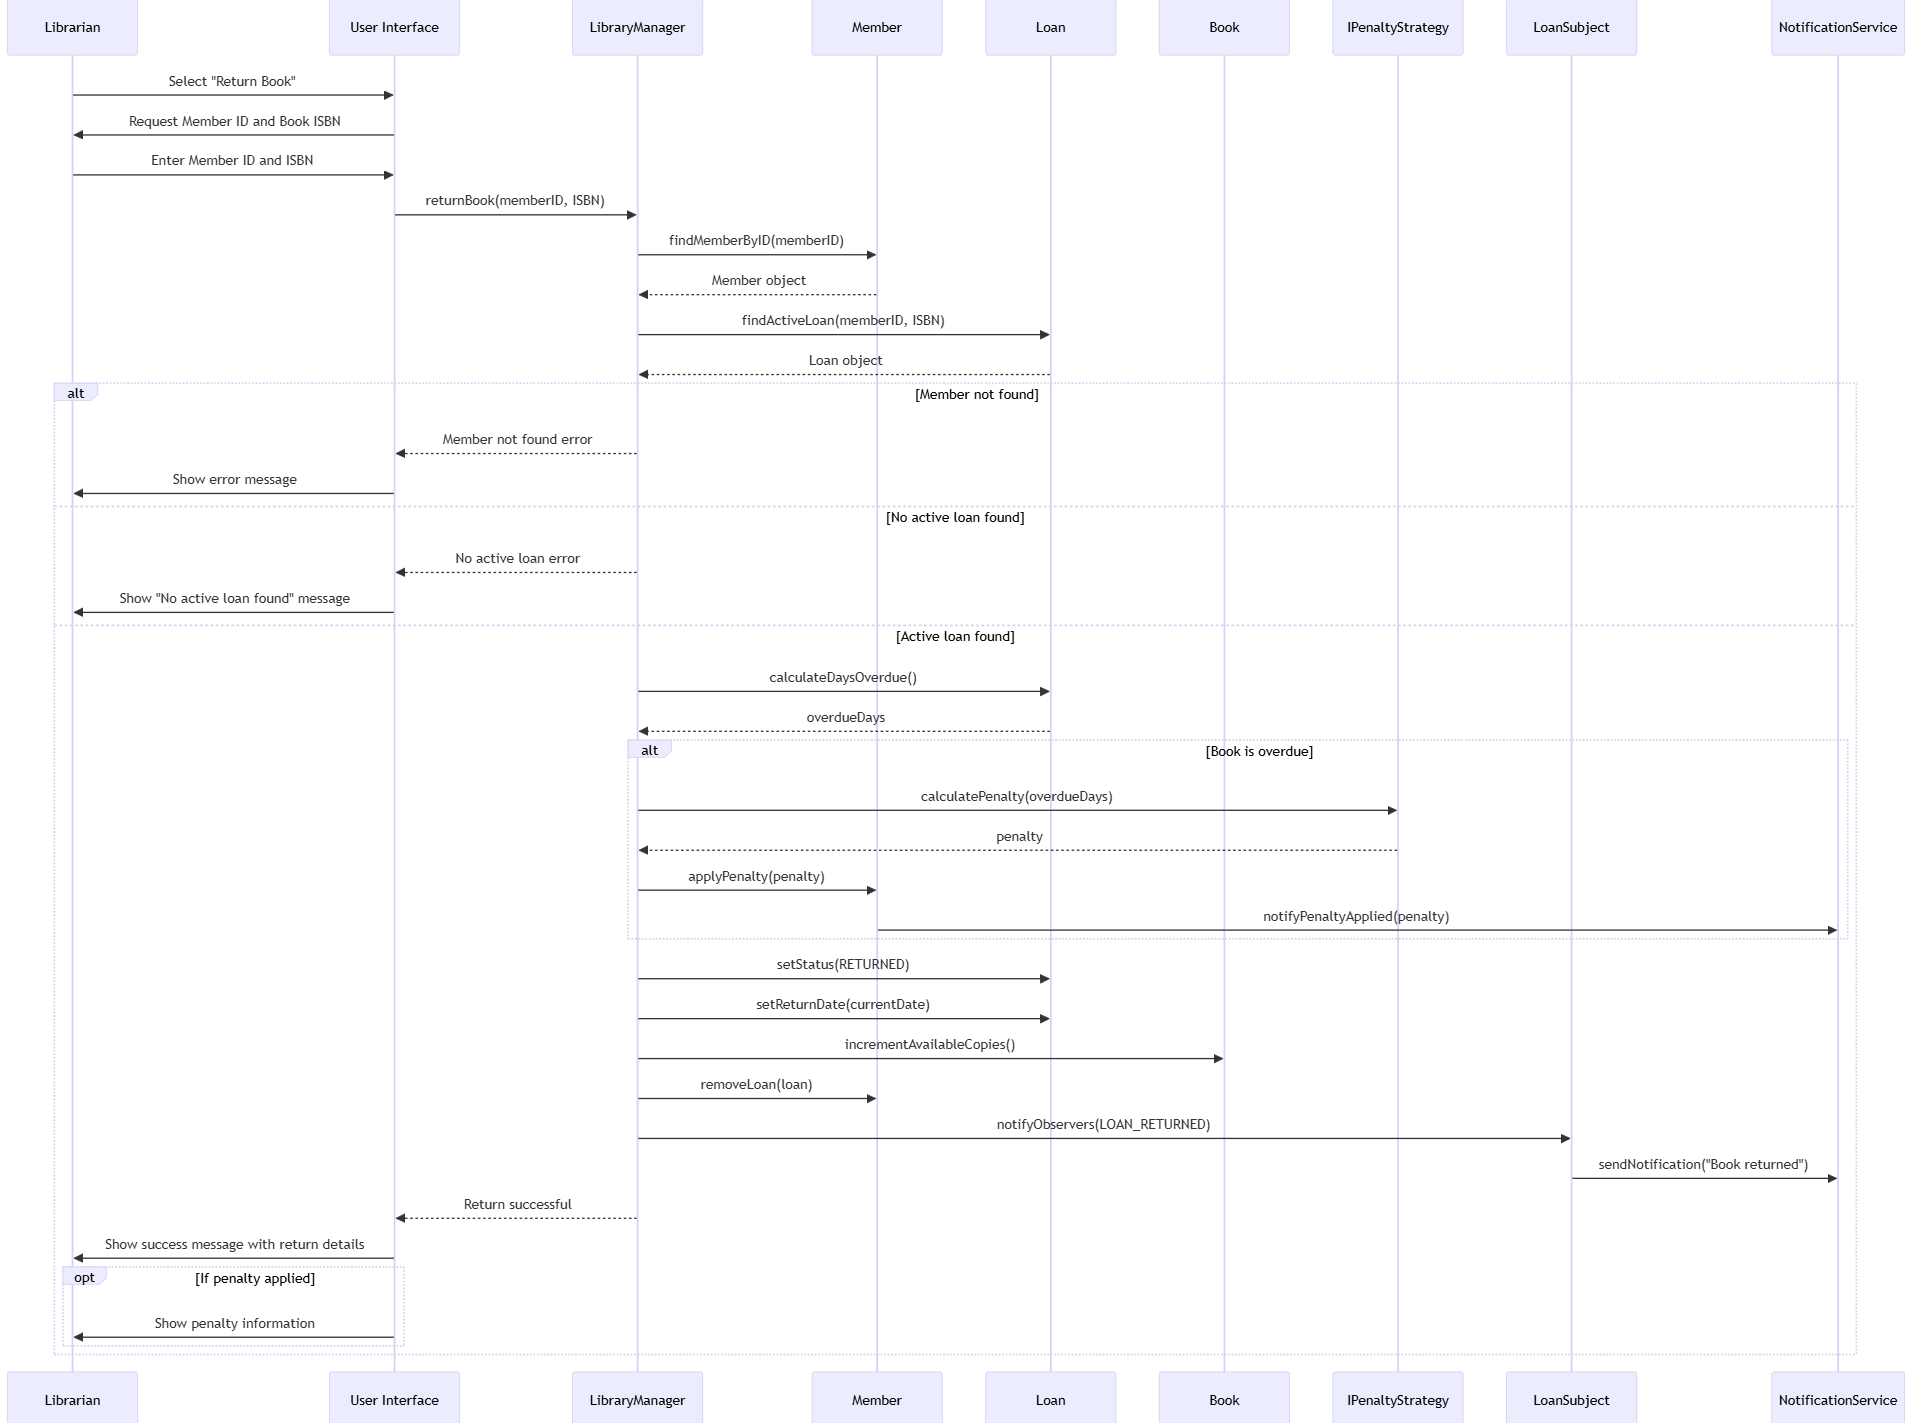
\includegraphics[width=\textwidth]{figures/sequence_return.png}
	\caption{Sequence Diagram for Returning a Book.}
	\label{fig:seq_return}
\end{figure}

\newpage

\subsection{User Interface Showcase}
The Library Management System features an intuitive graphical user interface built with Dear ImGui and DirectX9, providing users with a modern and user-friendly experience. The following screenshots demonstrate the various interfaces and functionalities available to both members and librarians.

\subsubsection{Authentication and Registration}
The system begins with secure user authentication, allowing users to either log in with existing credentials or register as new members.

\begin{figure}[H]
	\centering
	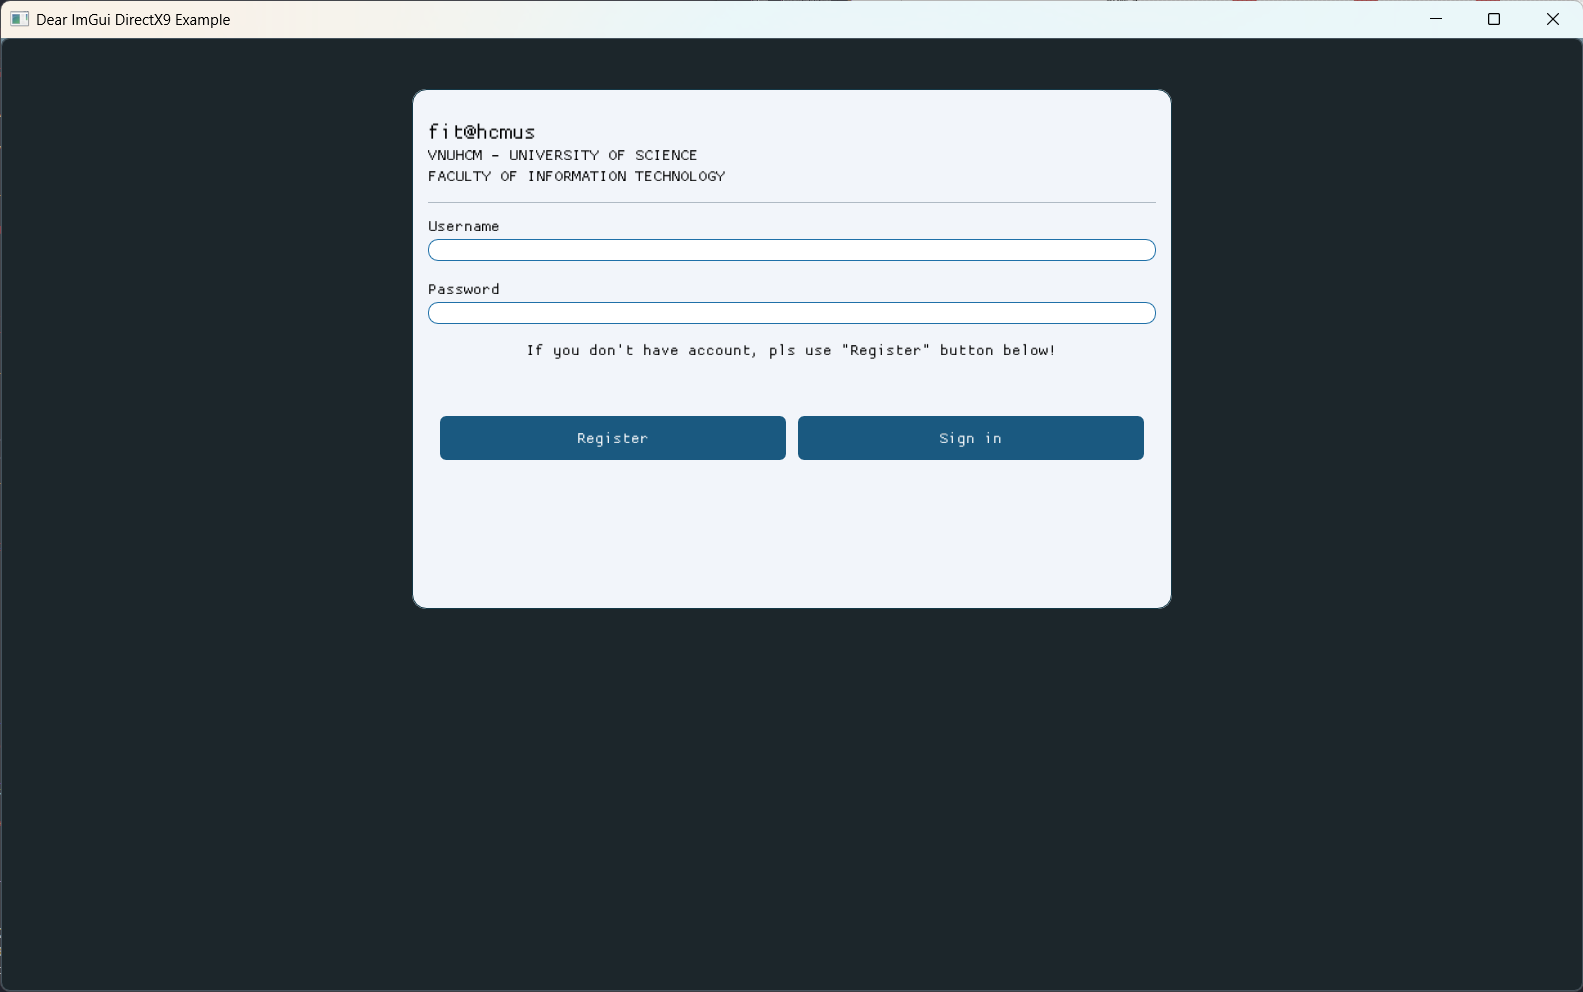
\includegraphics[width=0.8\textwidth]{figures/screenshot_login.png}
	\caption{User login interface with secure authentication.}
	\label{fig:ss_login}
\end{figure}

\begin{figure}[H]
	\centering
	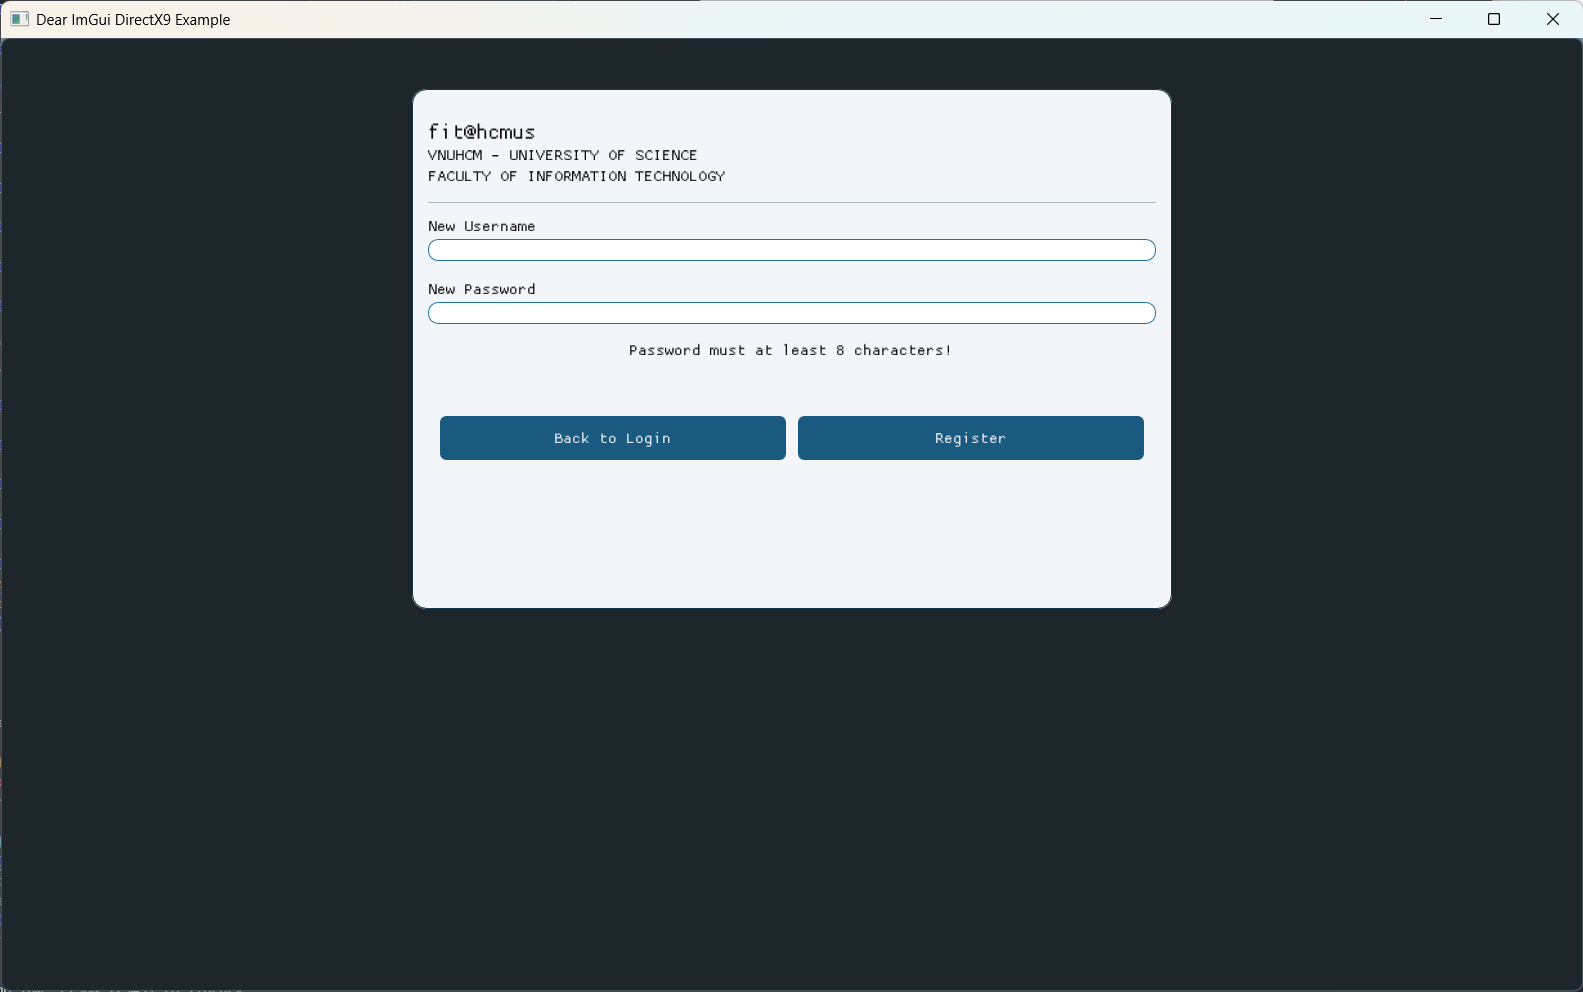
\includegraphics[width=0.8\textwidth]{figures/screenshot_register.png}
	\caption{New member registration form with input validation.}
	\label{fig:ss_register}
\end{figure}

\subsubsection{Member Interface}
Members have access to a clean and organized interface for browsing books, managing their loans, and viewing notifications.

\begin{figure}[H]
	\centering
	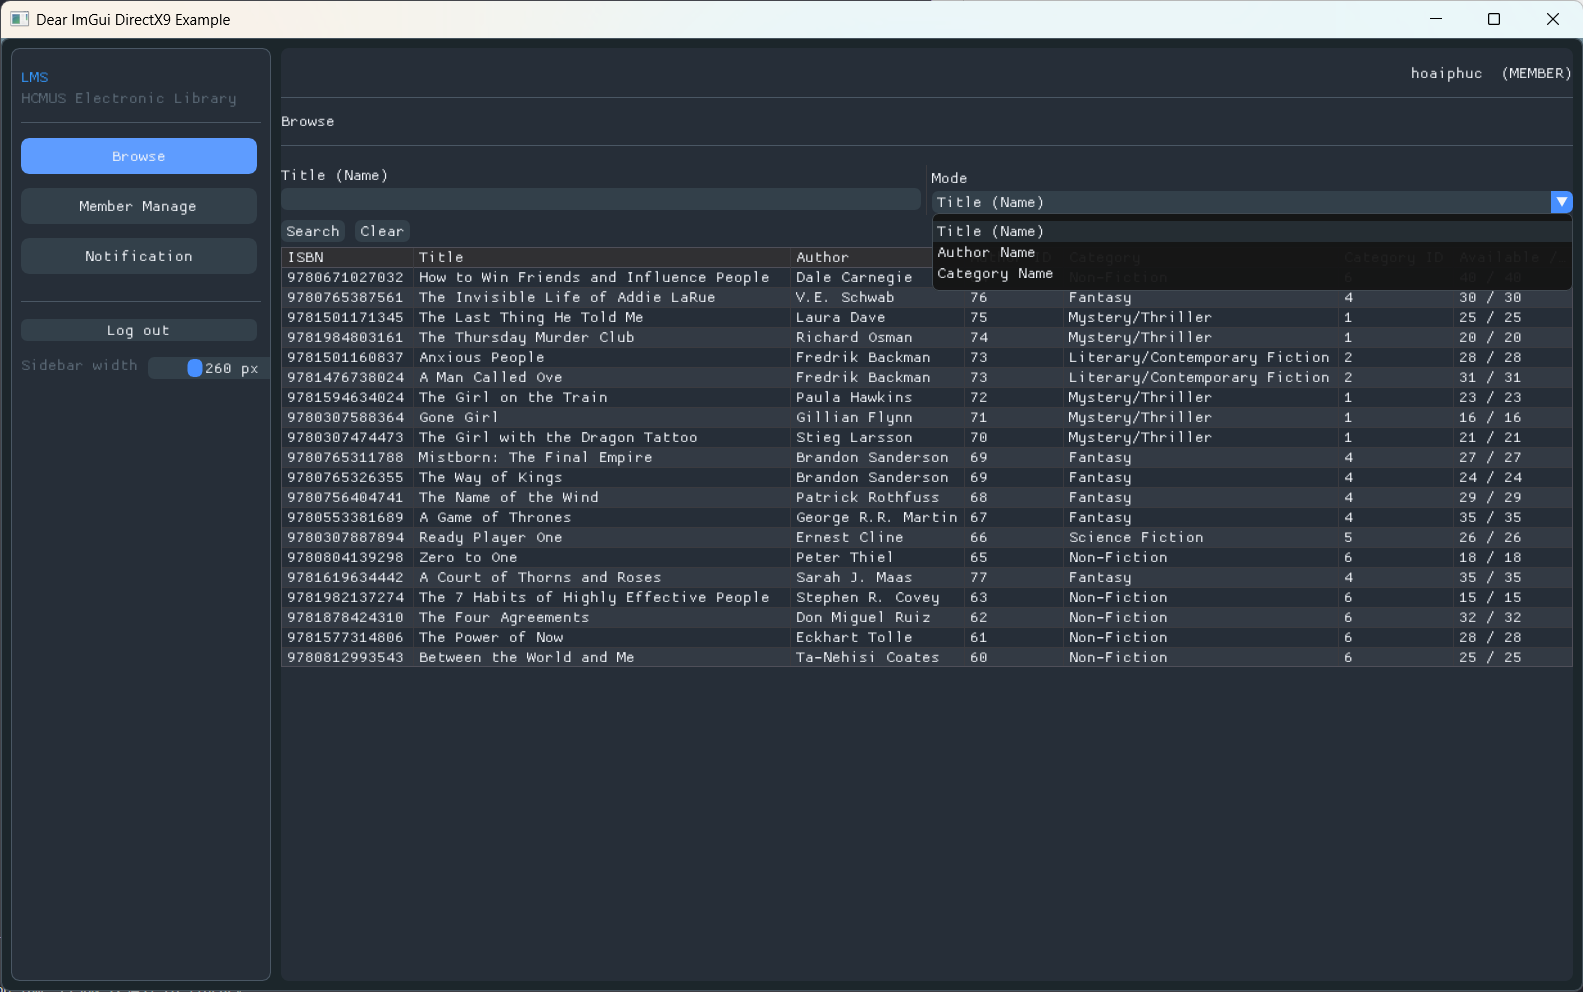
\includegraphics[width=0.9\textwidth]{figures/screenshot_member_browse.png}
	\caption{Member book browsing interface with search and filter options.}
	\label{fig:ss_member_browse}
\end{figure}

\begin{figure}[H]
	\centering
	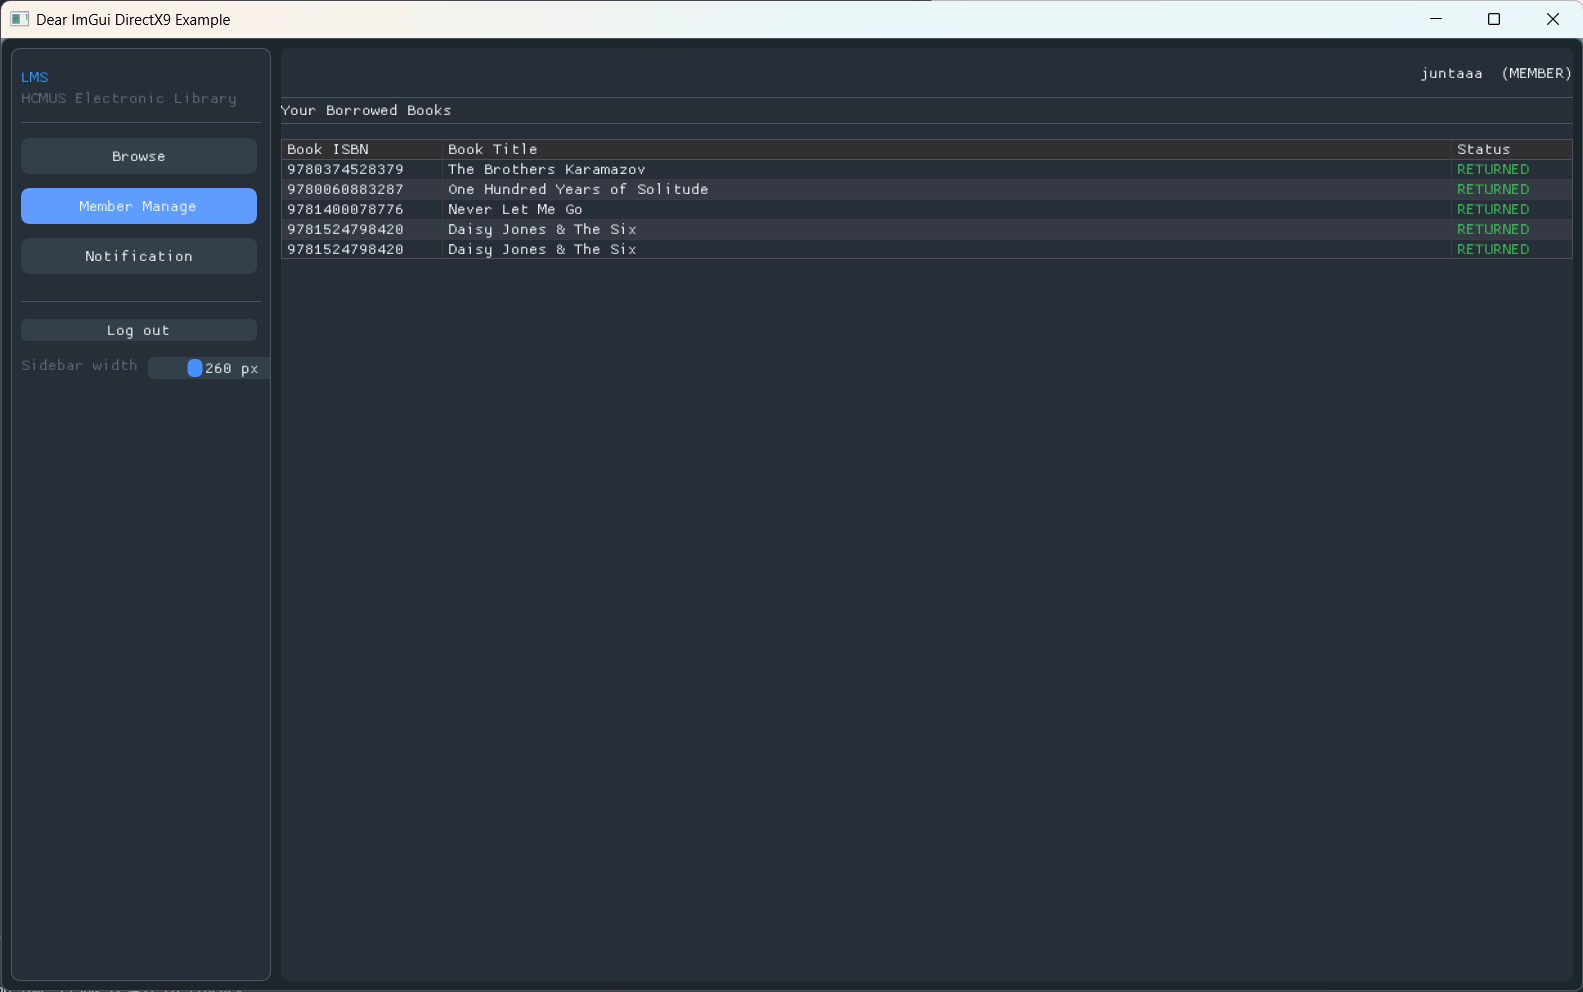
\includegraphics[width=0.9\textwidth]{figures/screenshot_member_myloanmanage.png}
	\caption{Member loan management showing current and past borrowings.}
	\label{fig:ss_member_loans}
\end{figure}

\begin{figure}[H]
	\centering
	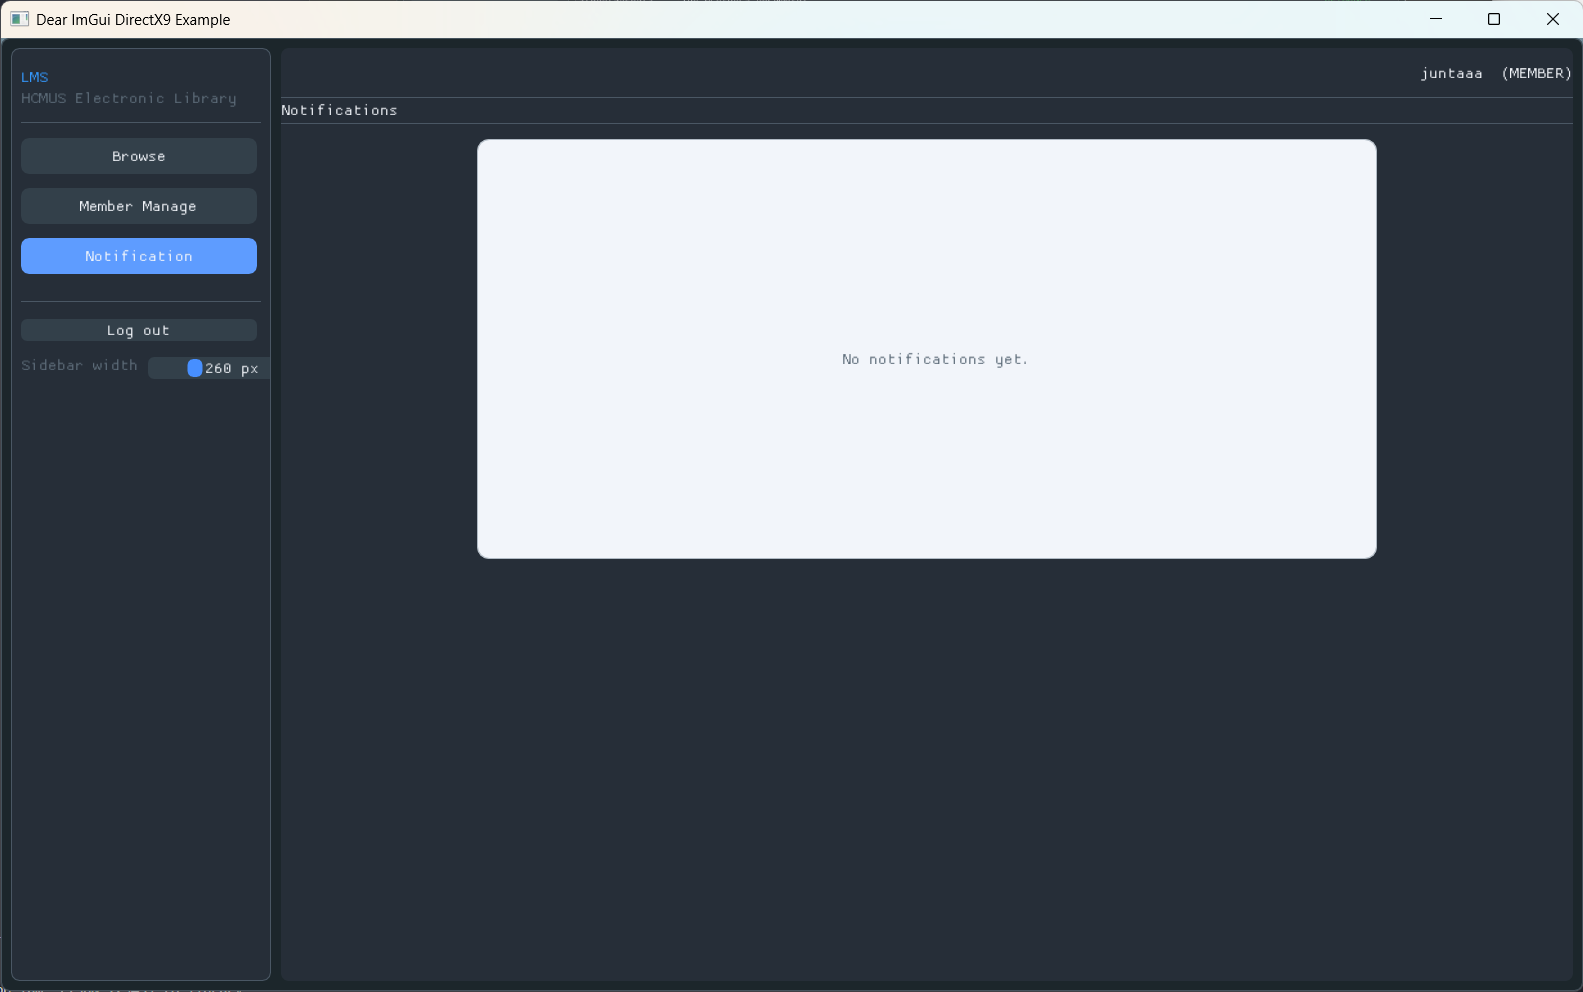
\includegraphics[width=0.9\textwidth]{figures/screenshot_member_noti.png}
	\caption{Member notification panel displaying important updates.}
	\label{fig:ss_member_noti}
\end{figure}

\subsubsection{Librarian Dashboard and Administration}
Librarians have access to a comprehensive dashboard with full administrative capabilities for managing the library system.

\begin{figure}[H]
	\centering
	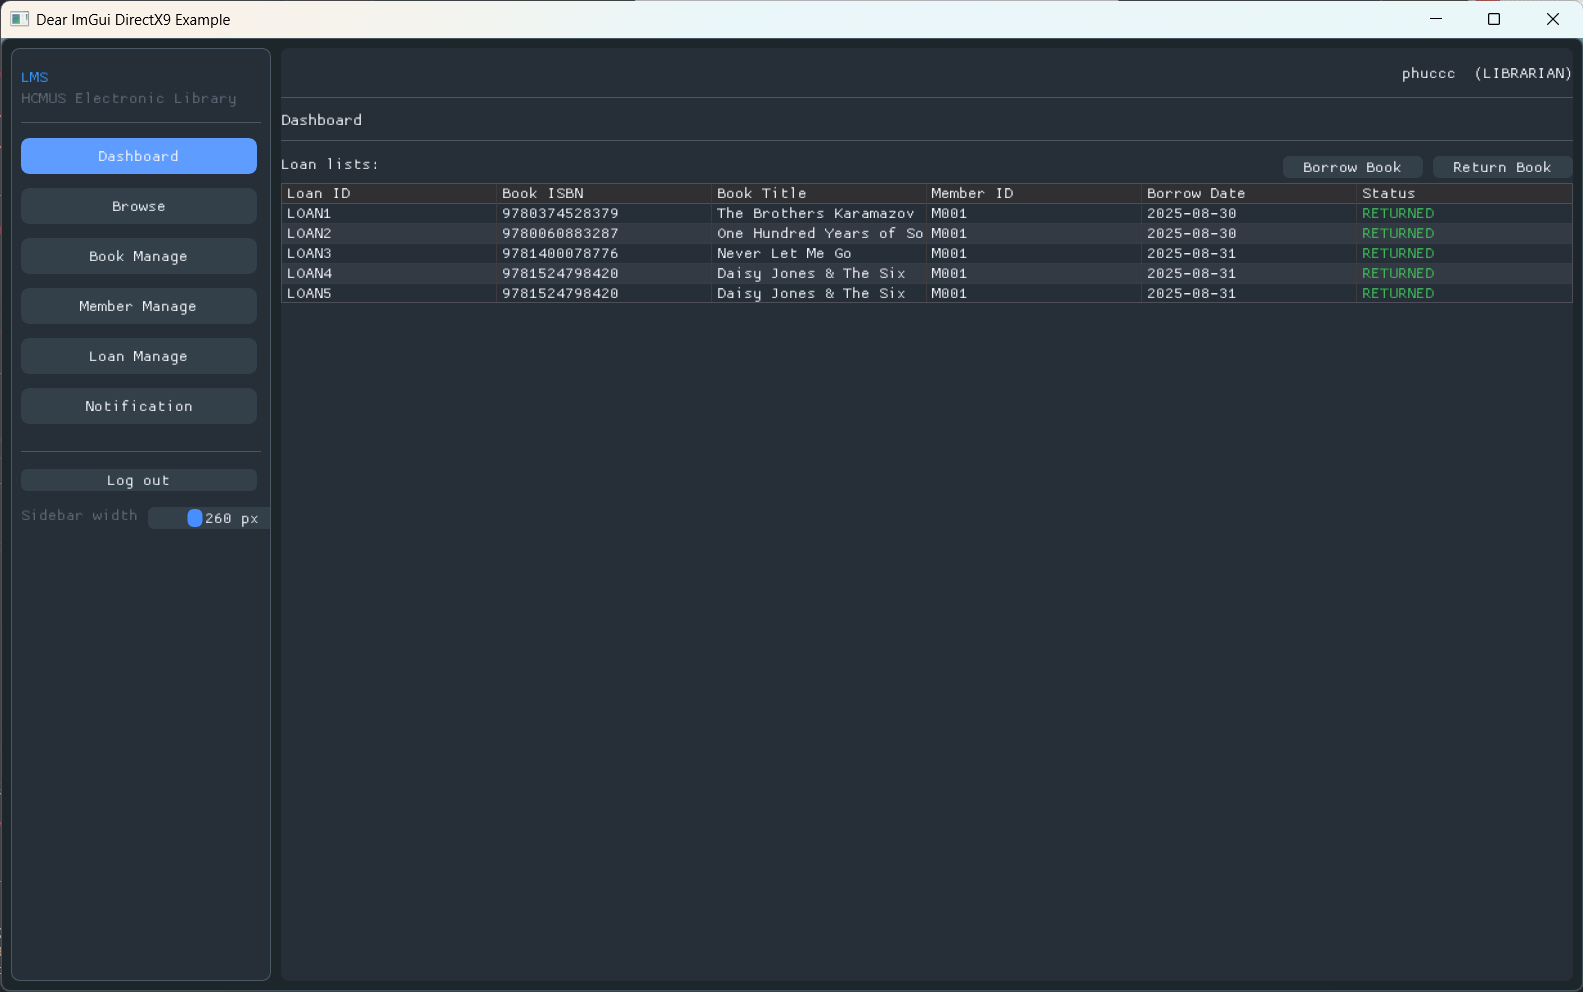
\includegraphics[width=\textwidth]{figures/screenshot_librarian_dashboard.png}
	\caption{Librarian dashboard overview with system statistics and quick actions.}
	\label{fig:ss_librarian_dashboard}
\end{figure}

\begin{figure}[H]
	\centering
	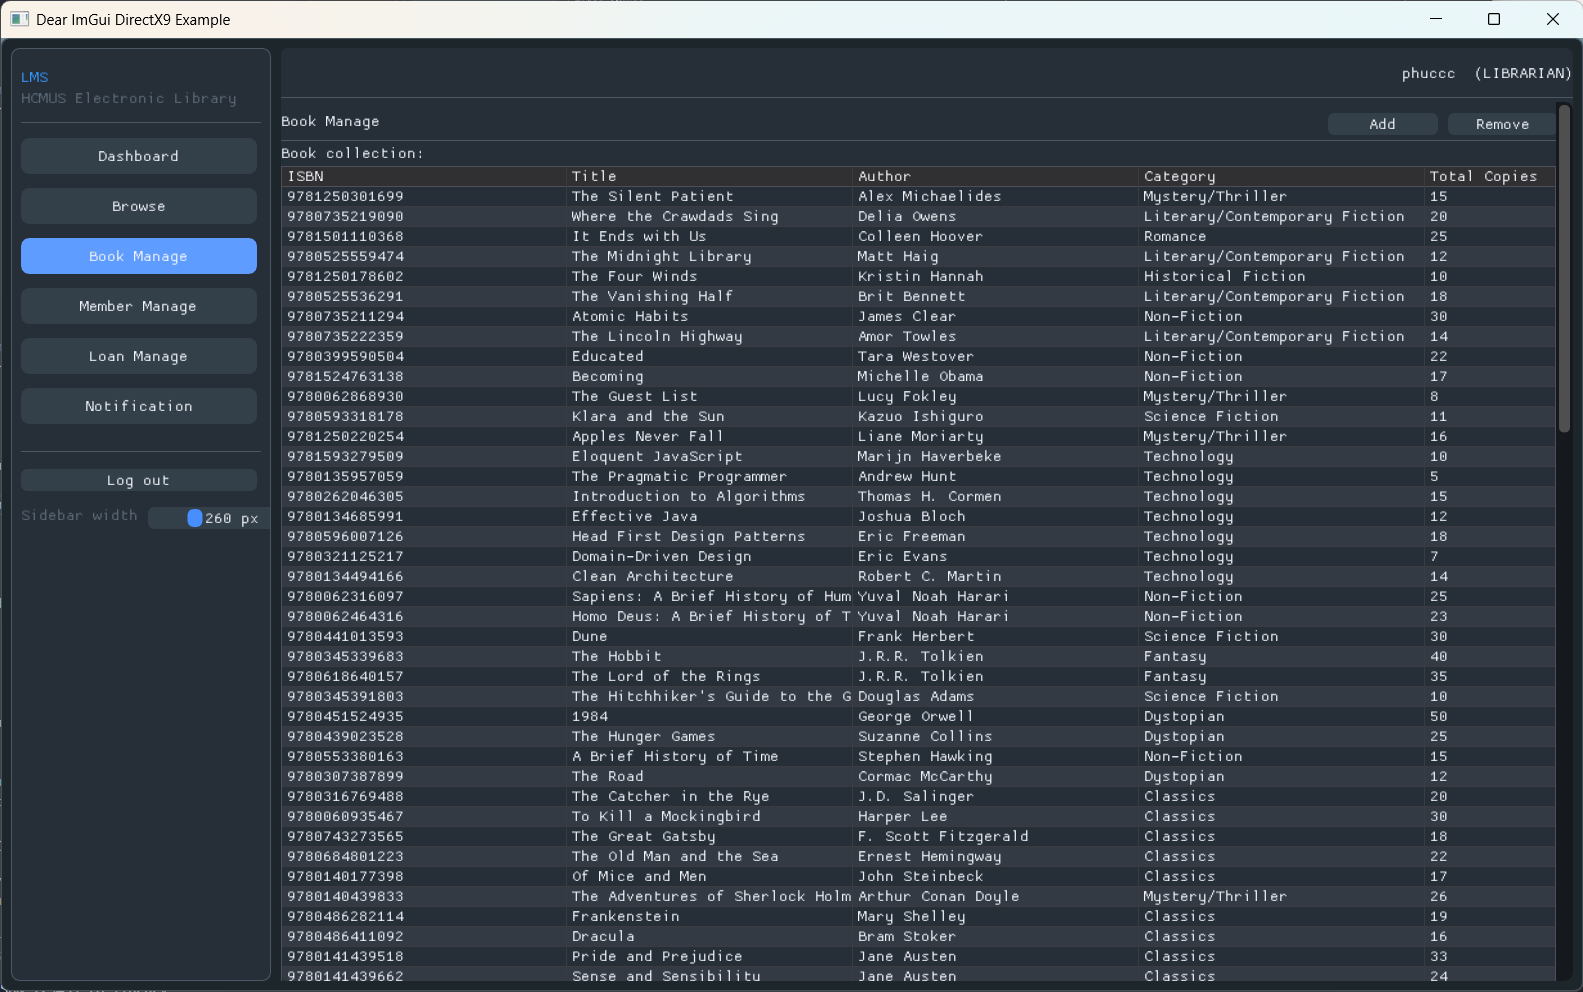
\includegraphics[width=0.9\textwidth]{figures/screenshot_librarian_bookmanage.png}
	\caption{Book management interface for librarians.}
	\label{fig:ss_librarian_bookmanage}
\end{figure}

\begin{figure}[H]
	\centering
	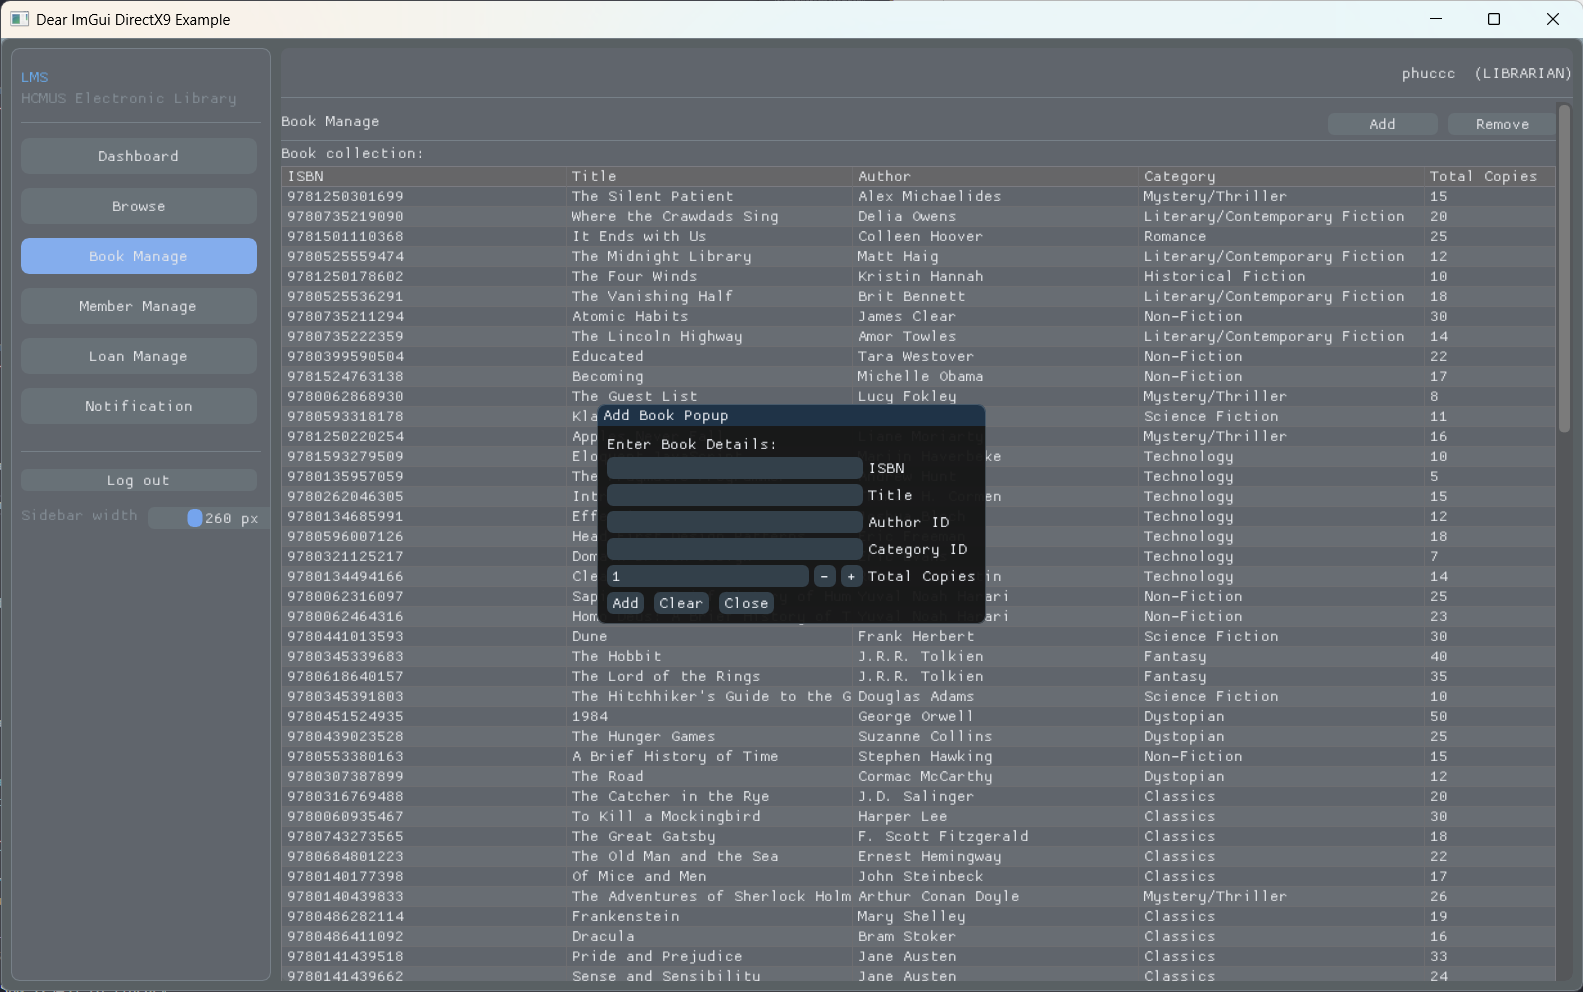
\includegraphics[width=0.9\textwidth]{figures/screenshot_librarian_addbook.png}
	\caption{Add new book form with comprehensive book information fields.}
	\label{fig:ss_librarian_addbook}
\end{figure}

\begin{figure}[H]
	\centering
	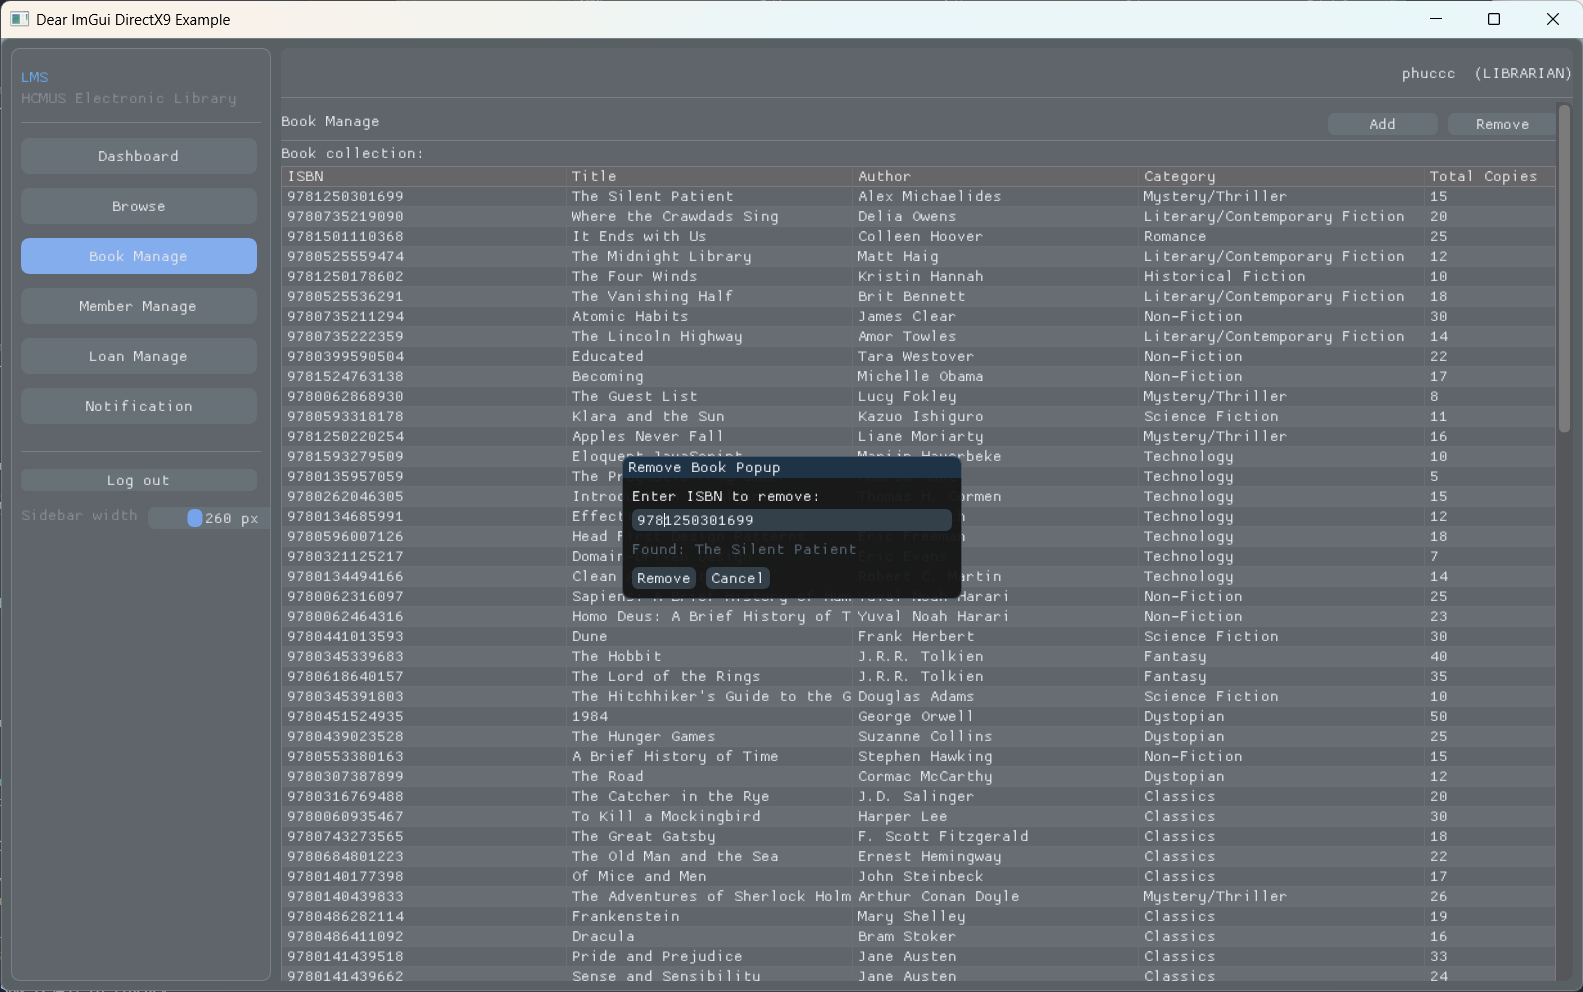
\includegraphics[width=0.9\textwidth]{figures/screenshot_librarian_removebook.png}
	\caption{Book removal interface with confirmation dialog.}
	\label{fig:ss_librarian_removebook}
\end{figure}

\subsubsection{Loan Management and Operations}
The system provides comprehensive loan management capabilities for librarians to track and manage all borrowing activities.

\begin{figure}[H]
	\centering
	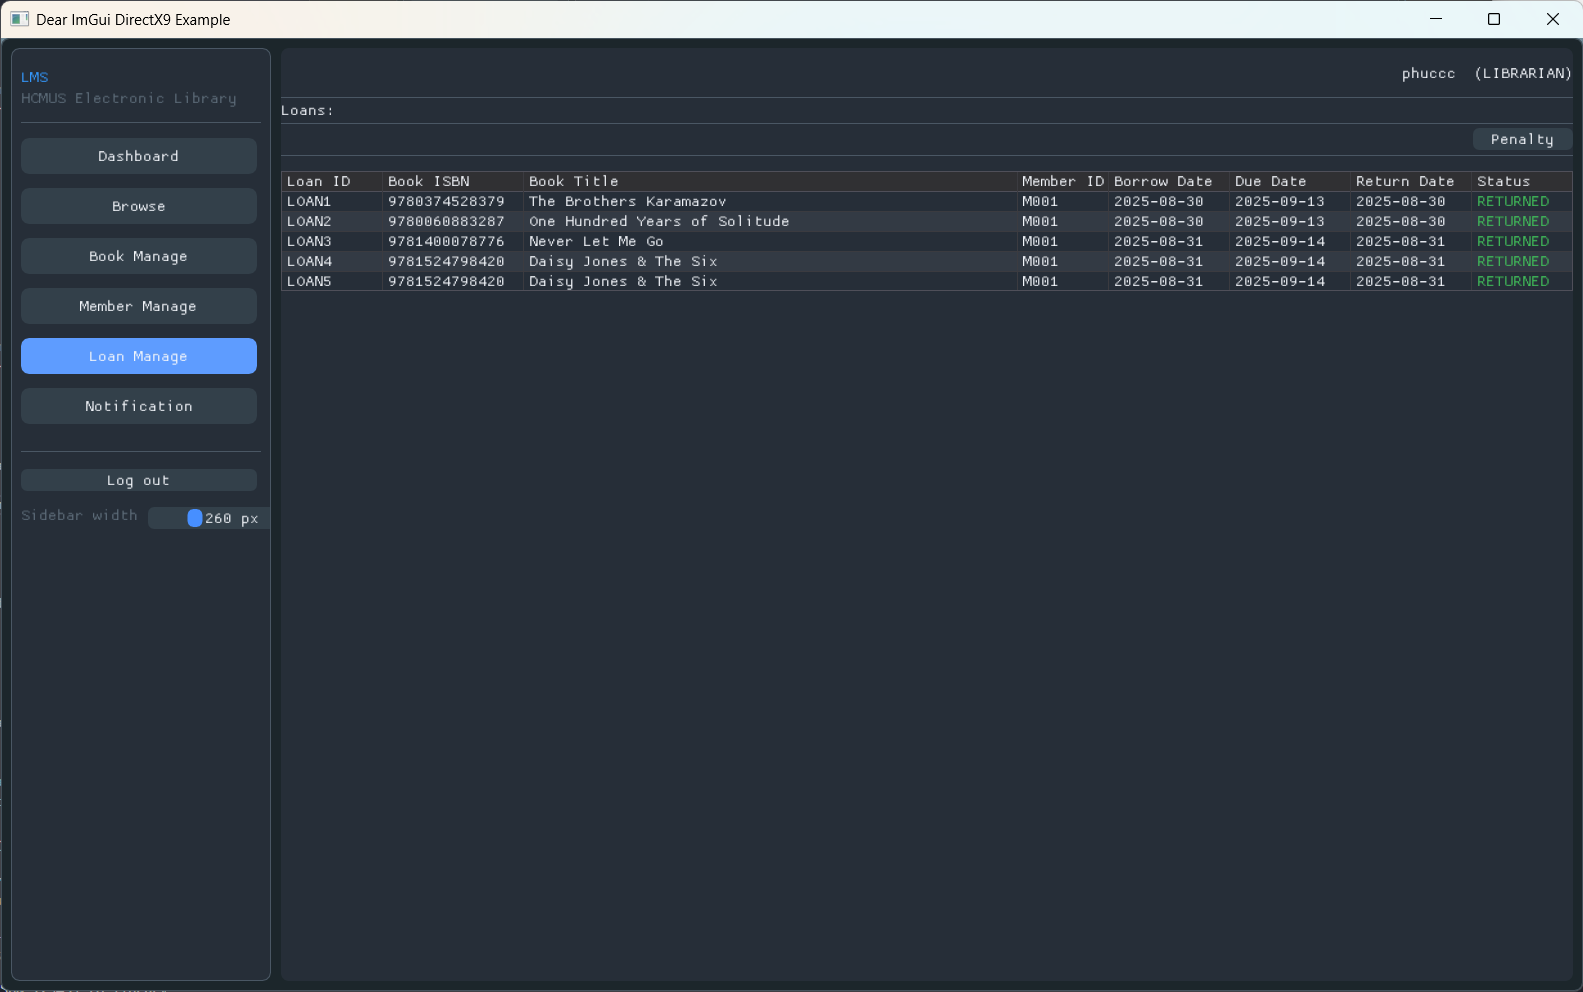
\includegraphics[width=0.9\textwidth]{figures/screenshot_librarian_loanmanage.png}
	\caption{Comprehensive loan management interface showing all active loans.}
	\label{fig:ss_librarian_loanmanage}
\end{figure}

\begin{figure}[H]
	\centering
	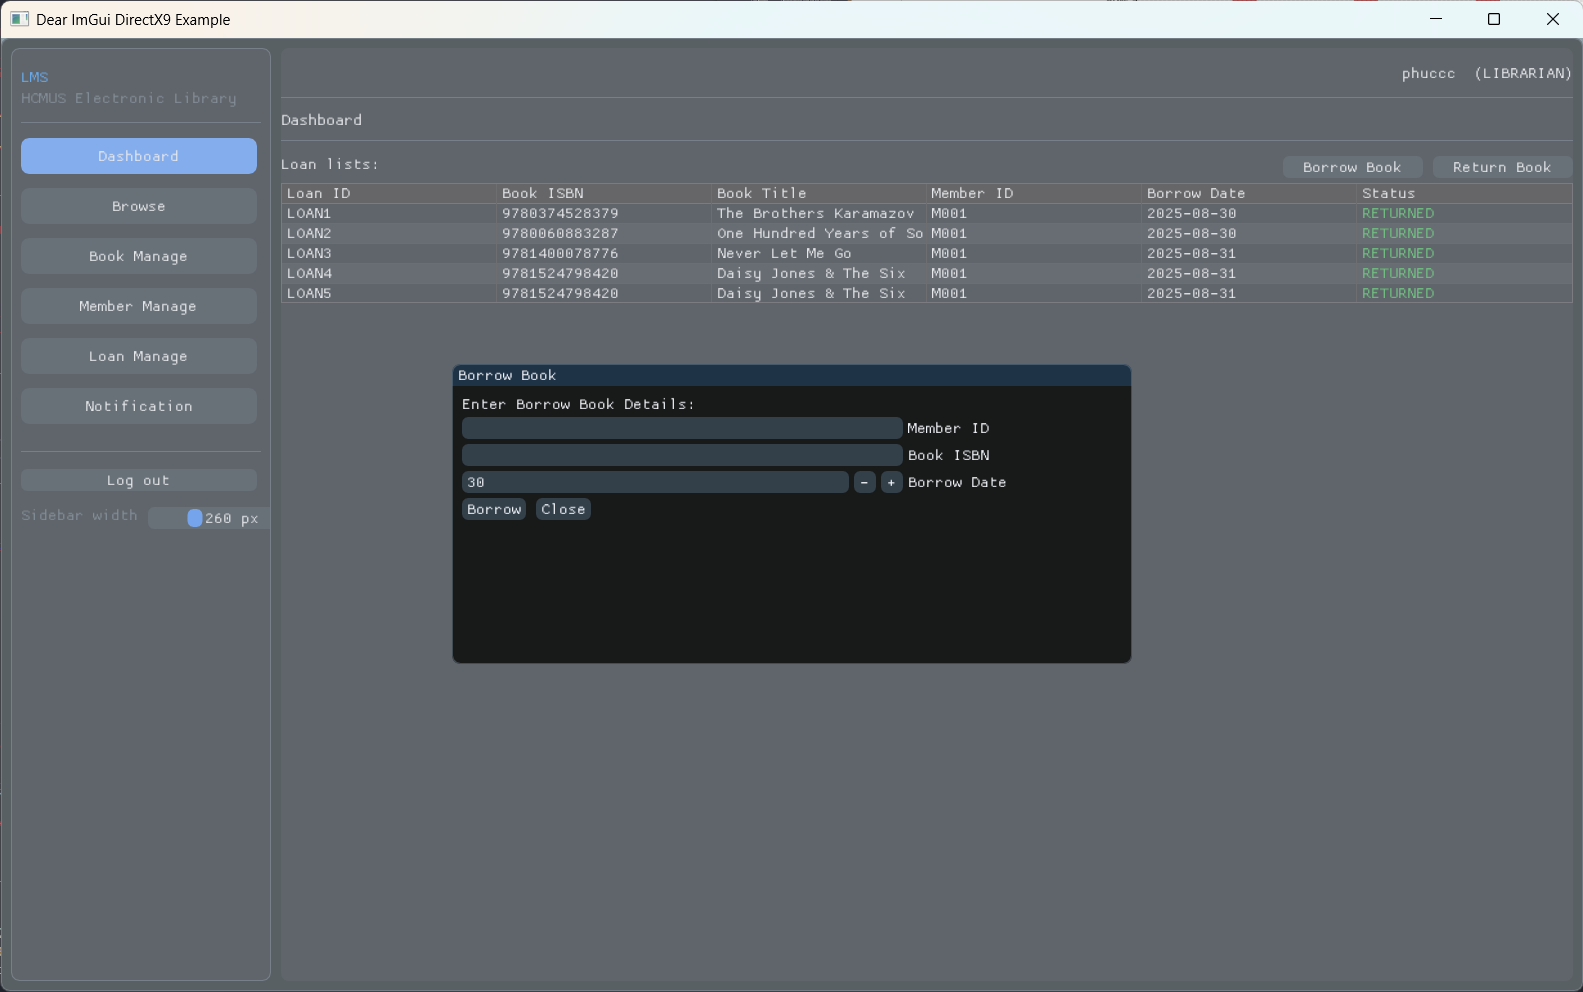
\includegraphics[width=0.9\textwidth]{figures/screenshot_librarian_borrow.png}
	\caption{Book borrowing interface for librarian-assisted transactions.}
	\label{fig:ss_librarian_borrow}
\end{figure}

\begin{figure}[H]
	\centering
	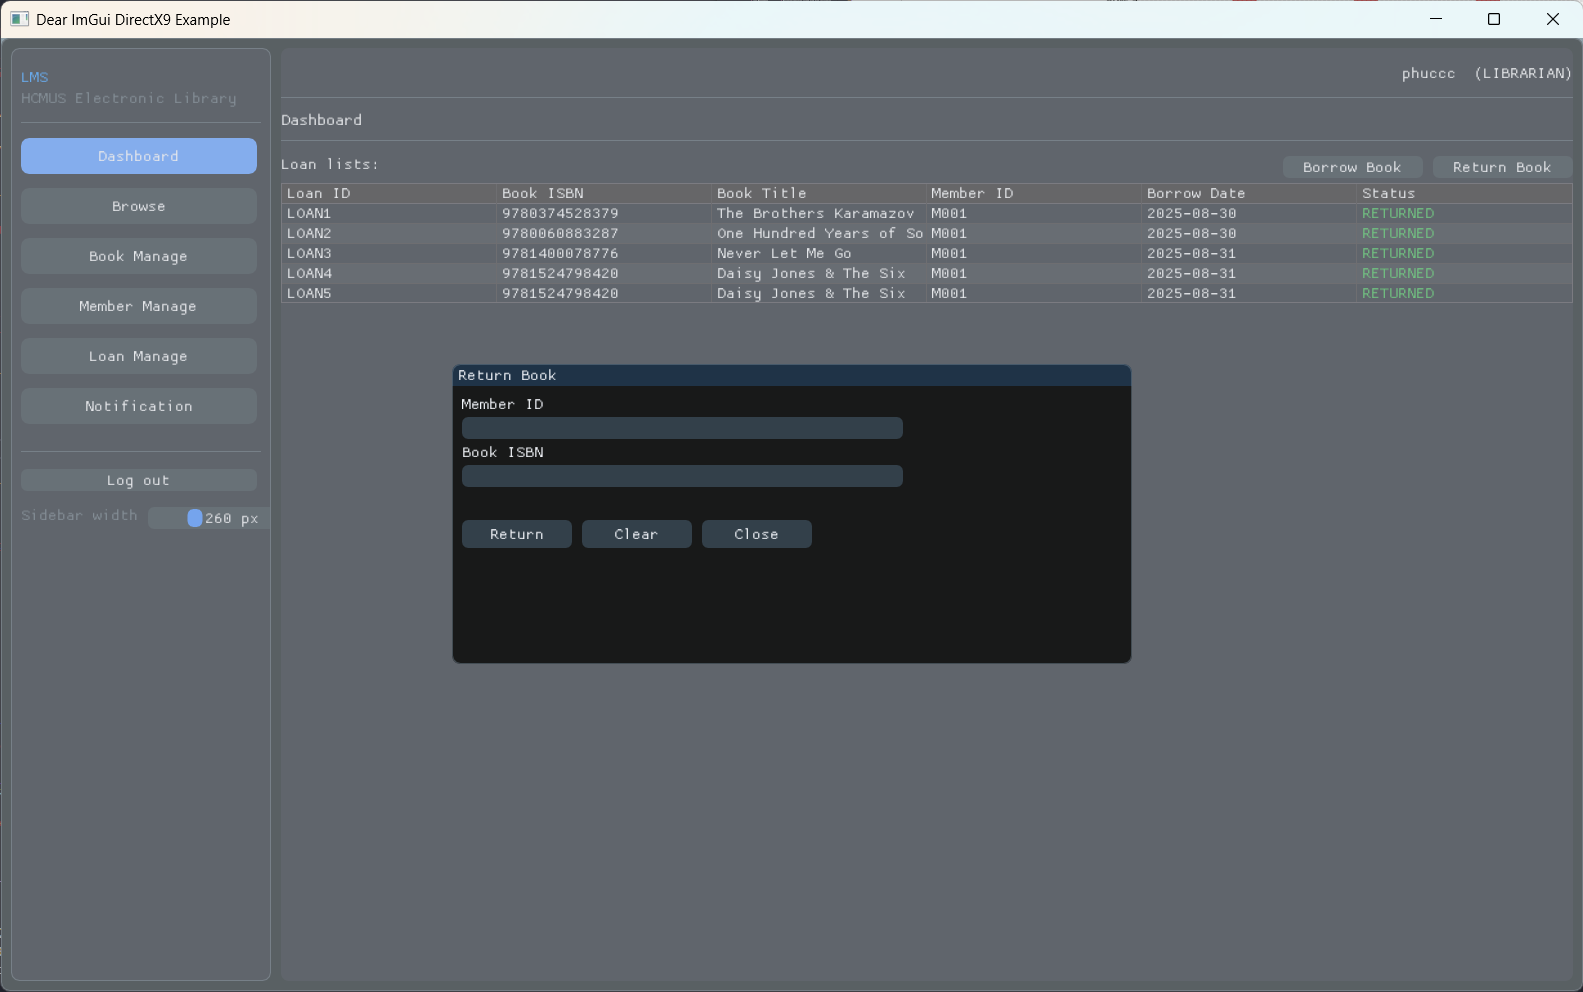
\includegraphics[width=0.9\textwidth]{figures/screenshot_librarian_return.png}
	\caption{Book return processing interface with loan status updates.}
	\label{fig:ss_librarian_return}
\end{figure}

\subsubsection{Member Management and System Administration}
Librarians can efficiently manage member accounts, handle penalties, and maintain system notifications.

\begin{figure}[H]
	\centering
	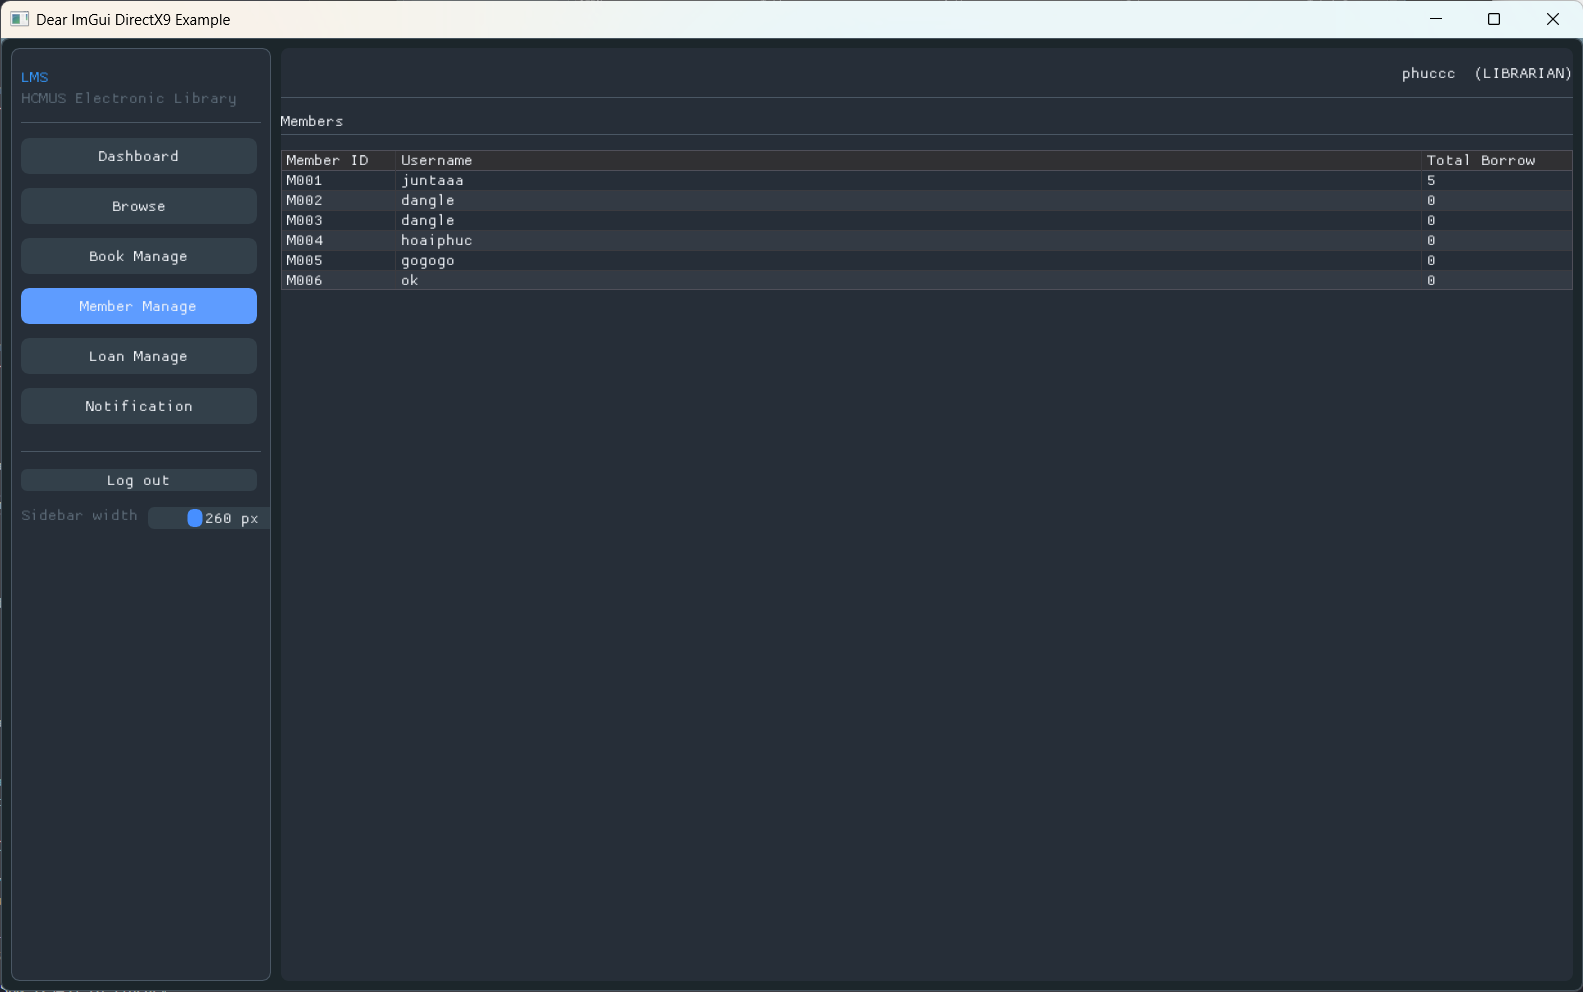
\includegraphics[width=0.9\textwidth]{figures/screenshot_librarian_memmanage.png}
	\caption{Member management interface for account administration.}
	\label{fig:ss_librarian_memmanage}
\end{figure}

\begin{figure}[H]
	\centering
	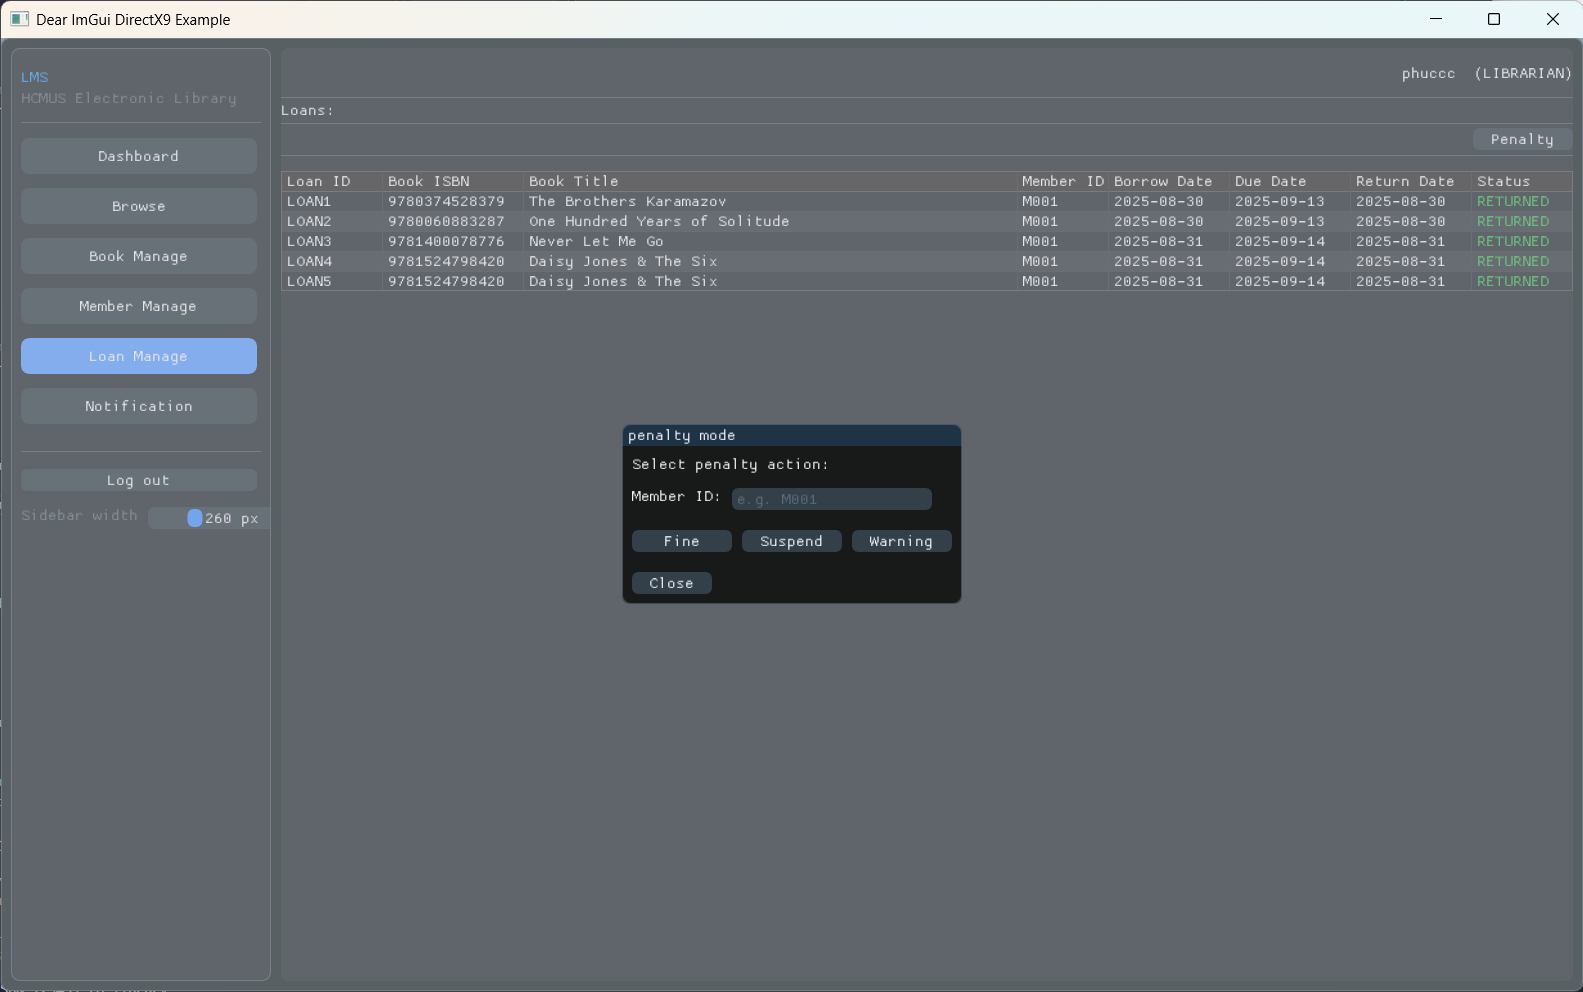
\includegraphics[width=0.9\textwidth]{figures/screenshot_librarian_penalty.png}
	\caption{Penalty management system for overdue books and fines.}
	\label{fig:ss_librarian_penalty}
\end{figure}

\begin{figure}[H]
	\centering
	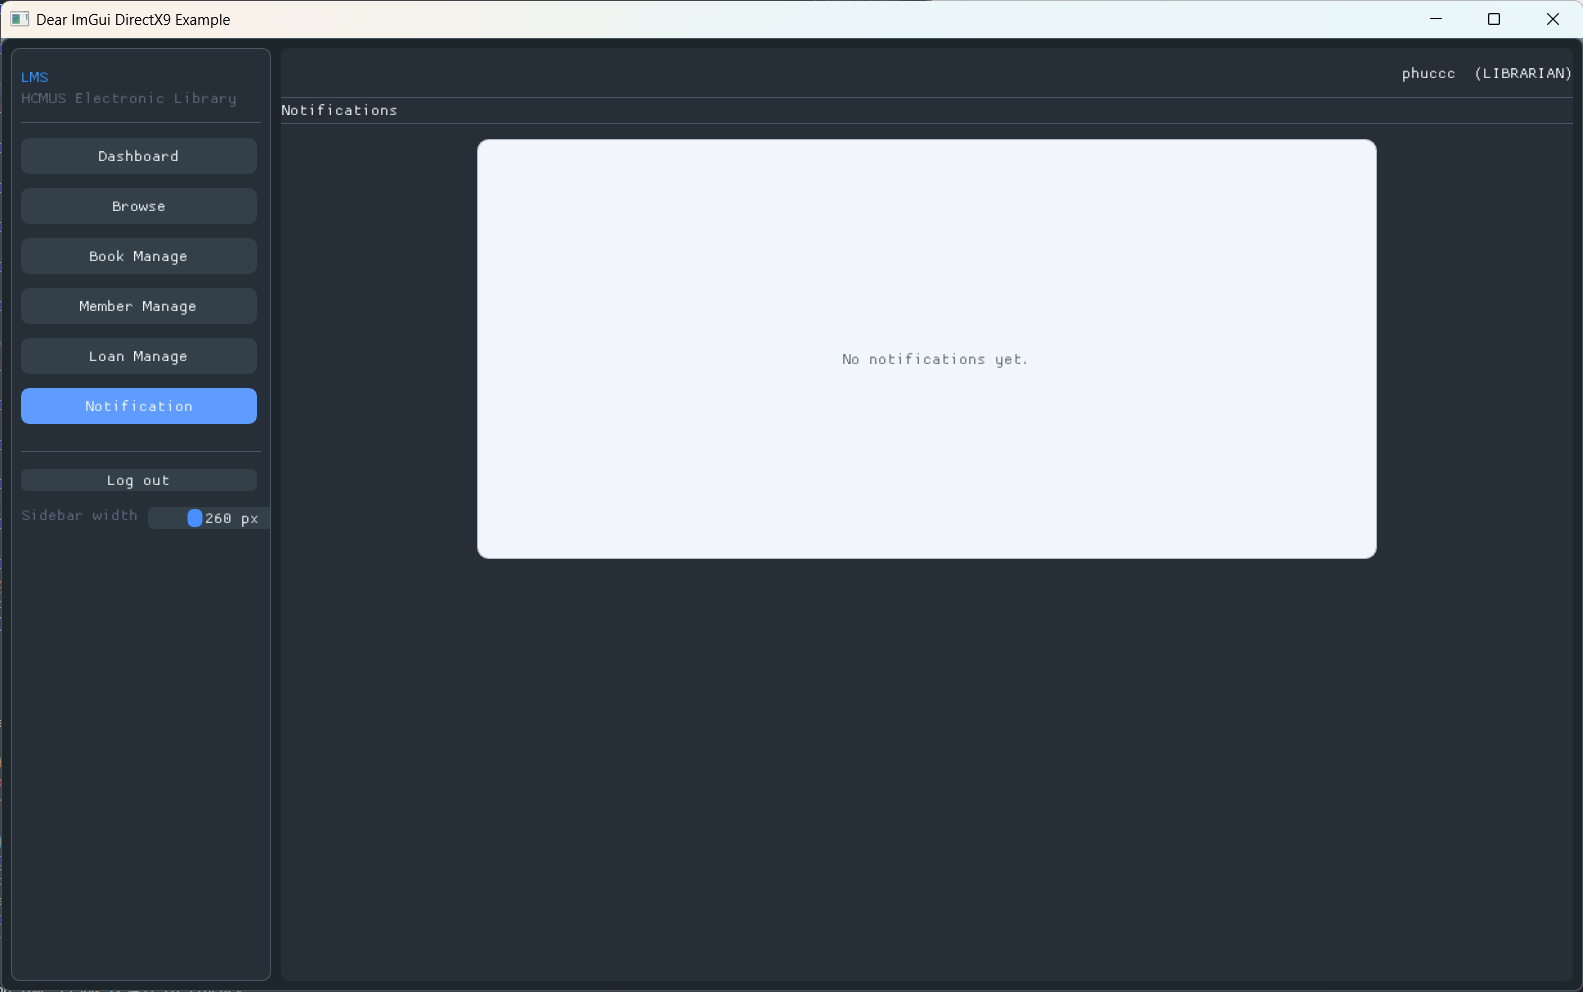
\includegraphics[width=0.9\textwidth]{figures/screenshot_librarian_noti.png}
	\caption{Librarian notification management for system-wide announcements.}
	\label{fig:ss_librarian_noti}
\end{figure}

\begin{figure}[H]
	\centering
	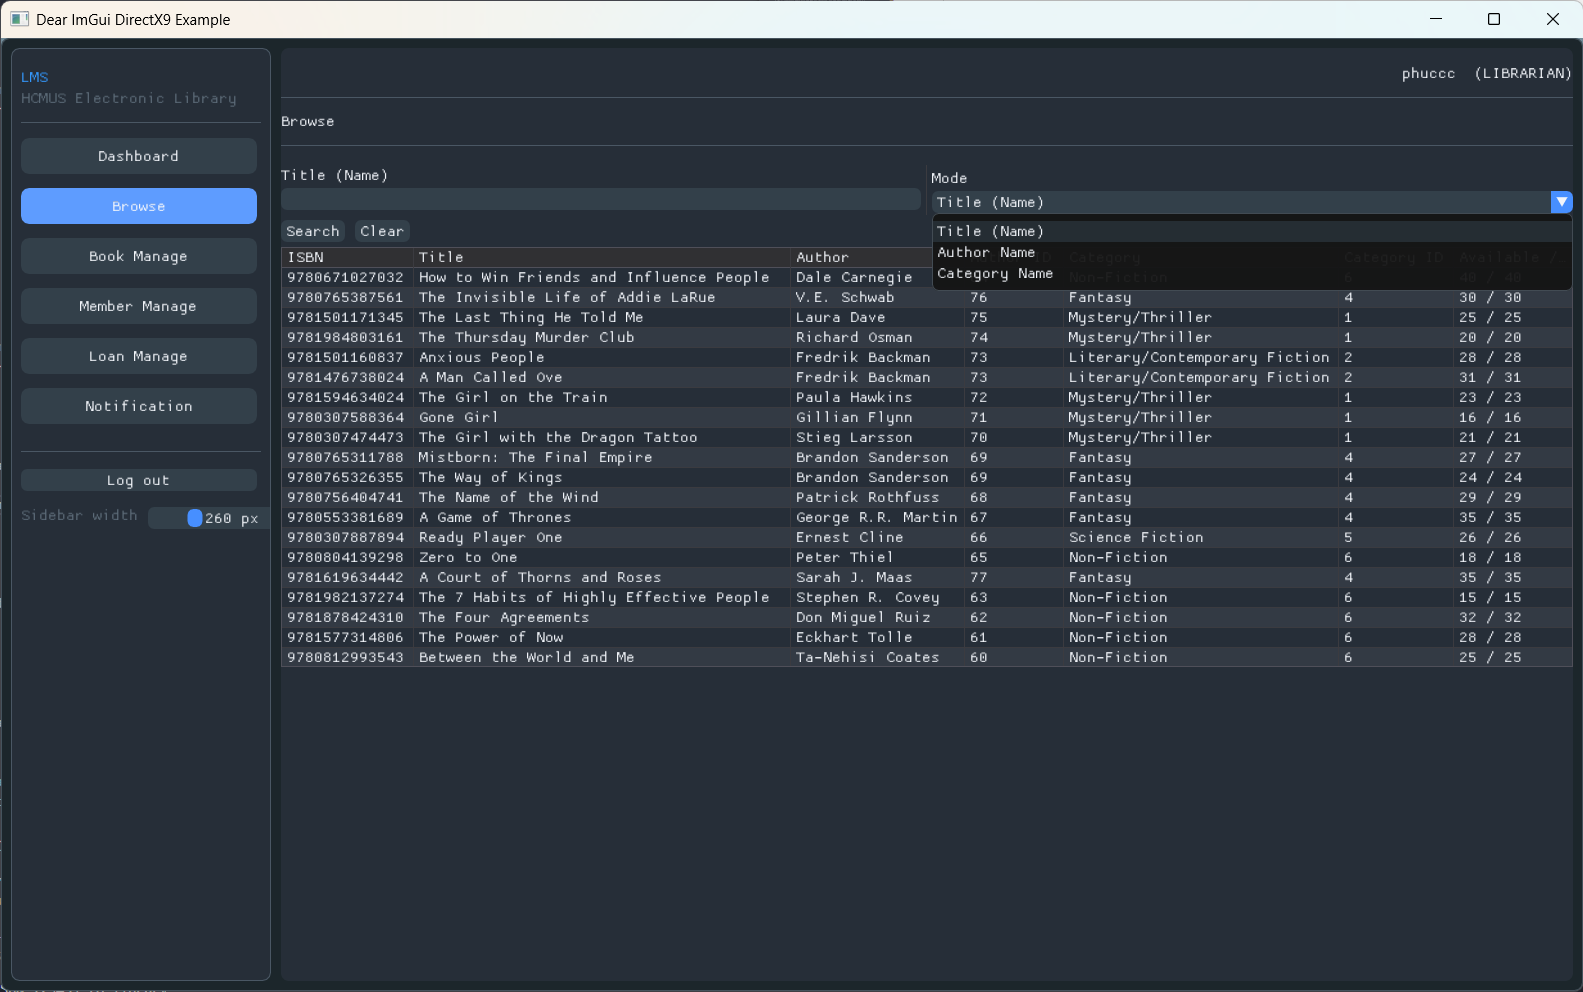
\includegraphics[width=0.9\textwidth]{figures/screenshot_librarian_browse.png}
	\caption{Librarian book browsing interface with advanced search capabilities.}
	\label{fig:ss_librarian_browse}
\end{figure}